%\documentclass[a4paper]{scrreprt}

%\usepackage[german]{babel}
%\usepackage[utf8]{inputenc}
%\usepackage[T1]{fontenc}
%\usepackage{ae}
%\usepackage{tocbasic}

%\begin{document}
     \subsection{Package edu.kit.pse.fridget.server.controllers}
     \begin{figure}[H]
	       \centering
	       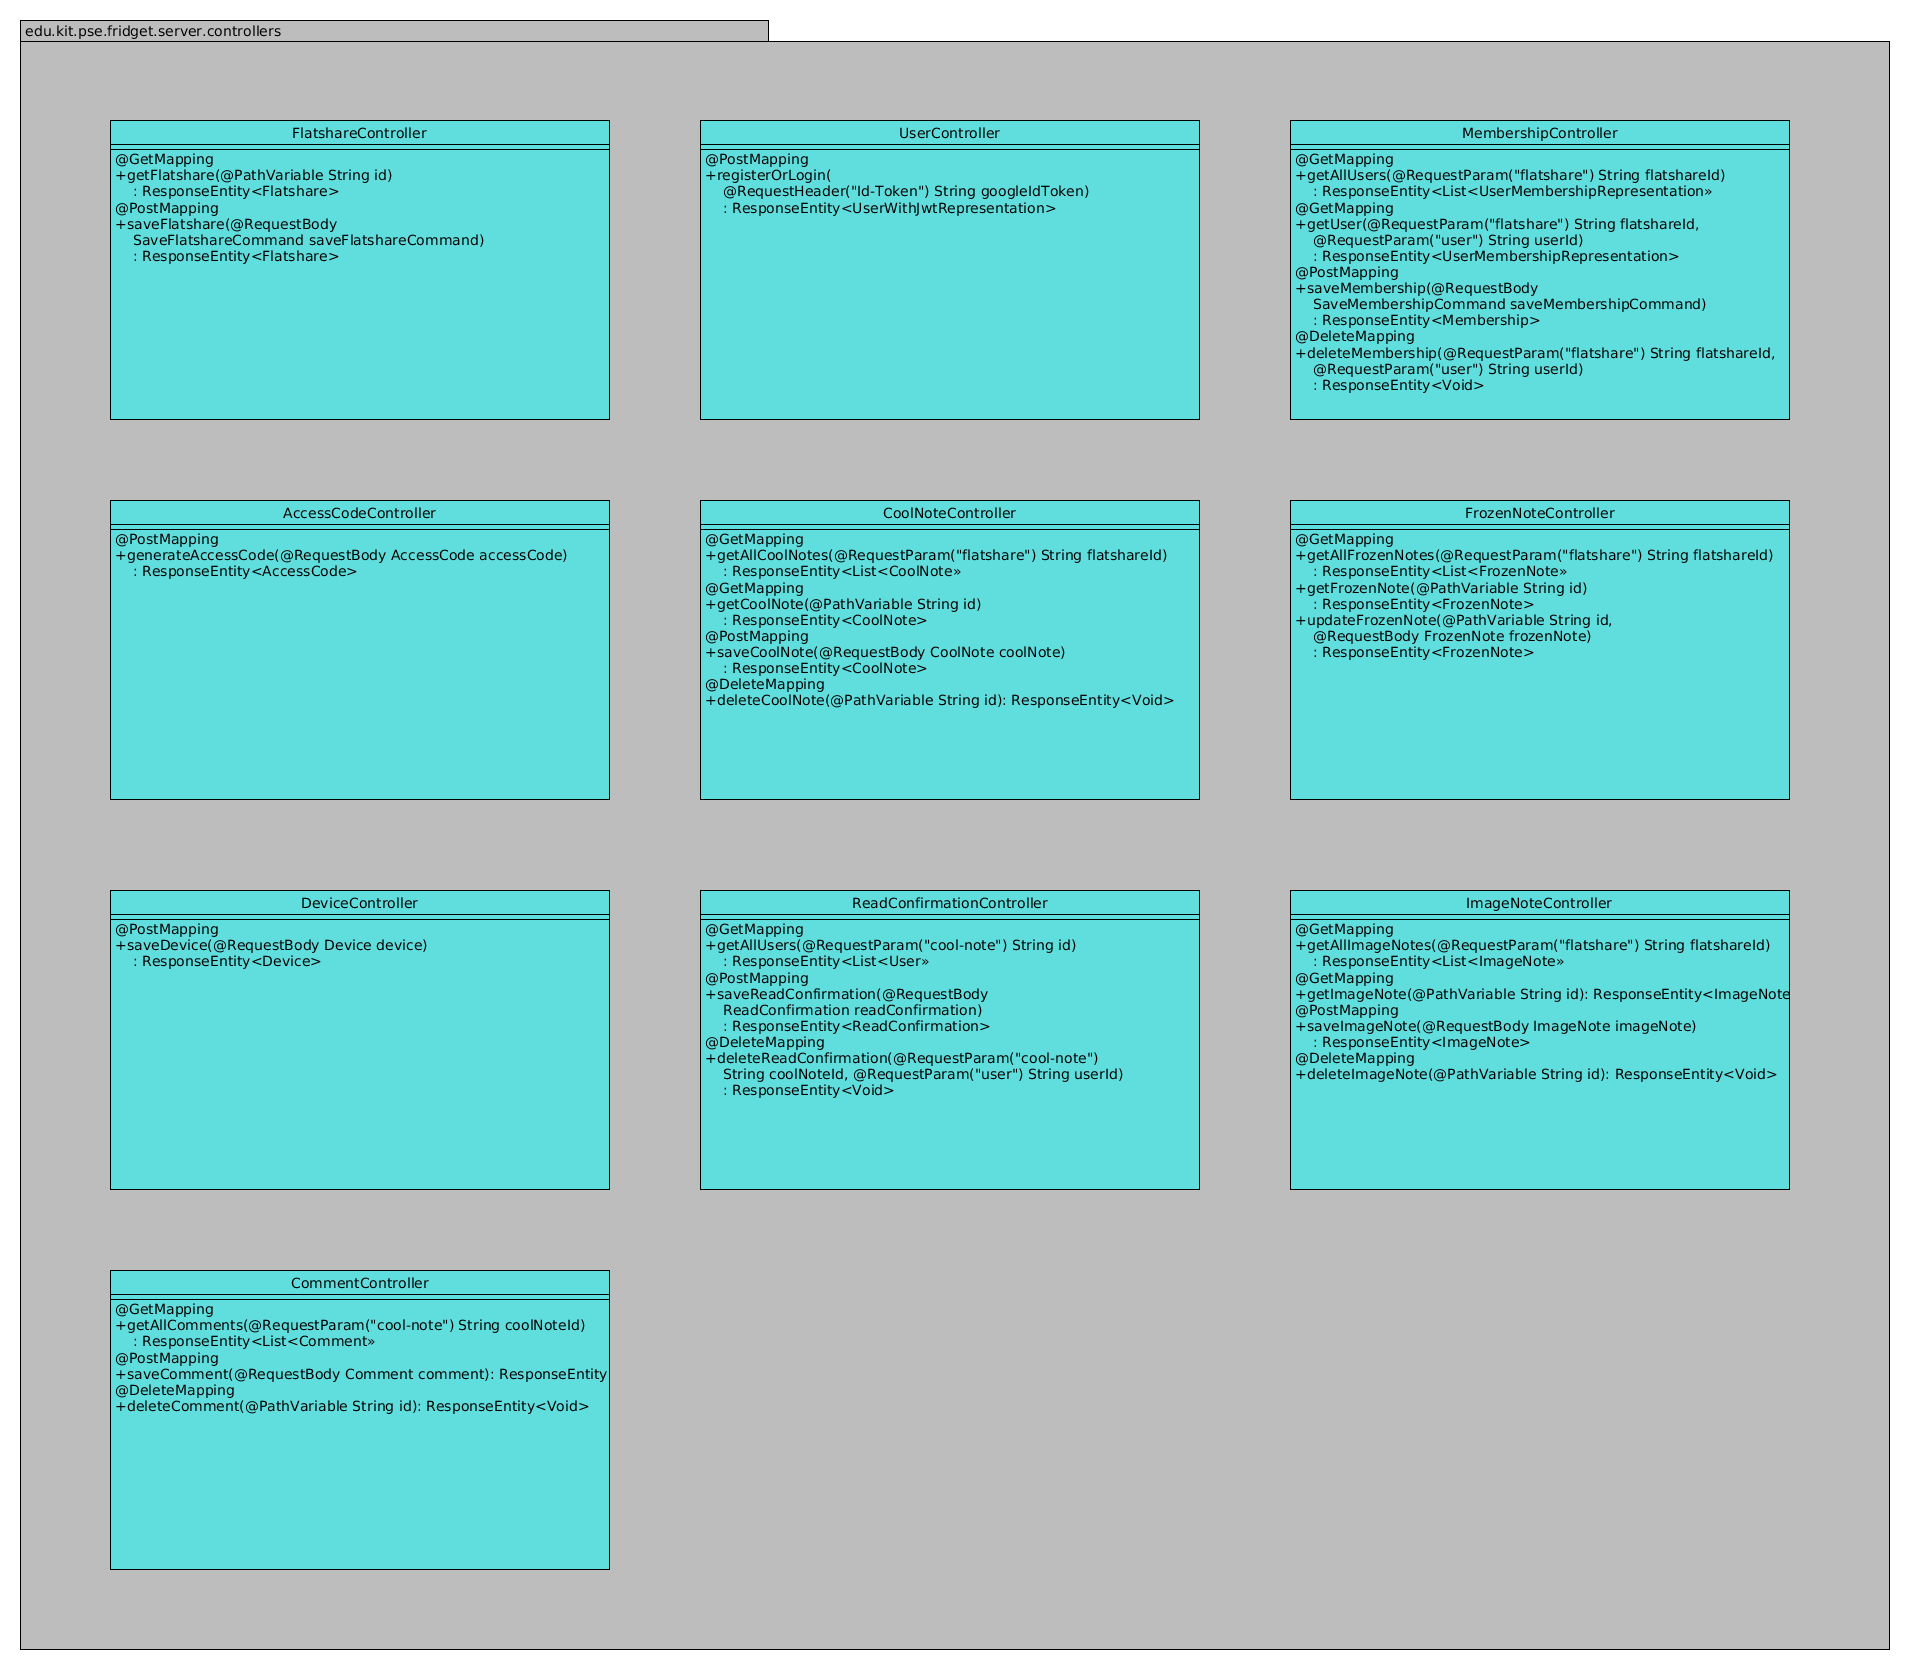
\includegraphics[scale = .25]{server-controllers.png}
	       \caption{Klassen des Controllers}
	      \end{figure}
     \subsubsection{\texttt{Class AccessCodeController}}
     \textbf{Beschreibung} \\
     \textit{Controller für Zugangscode}
     \paragraph*{Konstruktor}\mbox{} \\
     \texttt{public AccessCodeController(AccessCodeService service)}
     \paragraph*{Methoden}
     \begin{itemize}
     	\item{\texttt{public ResponseEntity<AccessCode> generateAccessCode(AccessCode accessCode)}}
     	
     	\textit{Generiert einen Zugangscode für eine WG.}
     	
     	\textbf{Parameter}
     	\begin{itemize}
     	\item\texttt{accessCode}\\
     	\textit{WG-ID mit leerem Zugangscode-Inhalt}
     	\end{itemize}
     	\textbf{Rückgabewert}\\
     	\begin{itemize}
     	\item\textit{Generierter Zugangscode als ResponseEntity}
     	\end{itemize}
     \end{itemize}
 
     \subsubsection{\texttt{Class CommentController}}
     \textbf{Beschreibung} \\
     \textit{Controller für Kommentar}
     \paragraph*{Konstruktor}\mbox{} \\
     \texttt{public CommentController(CommentService service)}
     \paragraph*{Methoden}
     \begin{itemize}
     	\item{\texttt{public ResponseEntity<List<Comment$>>$ getAllComments(String coolNoteId)}}
     	
     	\textit{Findet alle Kommentare zu einer Cool Note.}
     	
     	\textbf{Parameter}
     	\begin{itemize}
     		\item\texttt{coolNoteId}\\
     		\textit{CoolNote-ID}
     	\end{itemize}
     	
     	\textbf{Rückgabewert}
     	\begin{itemize}
     		\item\textit{Liste von gefundenen Kommentaren als ResponseEntity} 
     	\end{itemize}
     
     	\item{\texttt{public ResponseEntity<Comment> saveComment(Comment comment)}}
     	
     	\textit{Speichert einen Kommentar.}
     	
     	\textbf{Parameter}
     	\begin{itemize}
     		\item\texttt{comment}\\
     		\textit{Kommentar zum Speichern}
     	\end{itemize}
     	
     	\textbf{Rückgabewert}
     	\begin{itemize}
     		\item\textit{Gespeicherter Kommentar als ResponseEntity}
     	\end{itemize}        
     
     \item{\texttt{public ResponseEntity<Void> deleteComment(String id)}}
     	
     	\textit{Löscht einen Kommentar.}
     	
     	\textbf{Parameter}
     	\begin{itemize}
     		\item\texttt{id}\\
     		\textit{Kommentar-ID} 
     	\end{itemize}
     	
     	\textbf{Rückgabewert}
     	\begin{itemize}
     		\item\textit{Leere ResponseEntity} 
     	\end{itemize}
     \end{itemize}
 
     \subsubsection{\texttt{Class CoolNoteController}}
     \textbf{Beschreibung} \\
     \textit{Controller für Cool Note}
     \paragraph*{Konstruktor}\mbox{}
     \texttt{public CoolNoteController(CoolNoteService coolNoteService, TaggedUserService taggedUserService)}
     \paragraph*{Methoden}
     \begin{itemize}
     	\item{\texttt{public ResponseEntity<List<CoolNote$>>$ getAllCoolNotes(String flatshareId)}}
     	
     	\textit{Findet alle Cool Notes mit getaggten Benutzern in einer WG.}
     	
     	\textbf{Parameter}
     	\begin{itemize}
     		\item\texttt{flatshareId}\\
     		\textit{WG-ID}
     	\end{itemize}
     	
     	\textbf{Rückgabewert}
     	\begin{itemize}
     		\item\textit{Liste von gefundenen CoolNotes mit ID von getaggten Benutzern als ResponseEntity}
     	\end{itemize}
     
     \item{\texttt{public ResponseEntity<CoolNote> getCoolNote(String id)}}
     	
     	\textit{Findet eine Cool Note mit getaggten Benutzern.}
     	
     	\textbf{Parameter}
     	\begin{itemize}
     		\item\texttt{id}\\
     		\textit{CoolNote-ID}
     	\end{itemize}
     	
     	\textbf{Rückgabewert}
     	\begin{itemize}
     		\item\textit{Gefundene CoolNote mit ID von getaggten Benutzern als ResponseEntity} 
     	\end{itemize}
     	        
     \item{\texttt{public ResponseEntity<CoolNote> saveCoolNote(CoolNote coolNote)}}
     	
     	\textit{Speichert eine Cool Note and die getaggten Benutzer.}
     	
     	\textbf{Parameter}
     	\begin{itemize}
     		\item\texttt{coolNote}\\
     		\textit{CoolNote zum speichern} 
     	\end{itemize}
     	
     	\textbf{Rückgabewert}
     	\begin{itemize}
     		\item\textit{Gespeicherte CoolNote als ResponseEntity}
     	\end{itemize}
          	        
     \item{\texttt{public ResponseEntity<Void> deleteCoolNote(String id)}}
     	
     	\textit{Löscht eine Cool Note.}
     	
     	\textbf{Parameter}
     	\begin{itemize}
     		\item\texttt{id}\\
     		\textit{CoolNote-ID}
     	\end{itemize}
     	
     	\textbf{Rückgabewert}
     	\begin{itemize}
     		\item\textit{Leere ResponseEntity}
     	\end{itemize}
     \end{itemize}
 
     \subsubsection{\texttt{Class DeviceController}}
     \textbf{Beschreibung} \\
     \textit{Controller für Gerät}
     \paragraph*{Konstruktor}\mbox{} \\
     \texttt{public DeviceController(DeviceService service)}
     \paragraph*{Methoden}
     \begin{itemize}
     	\item{\texttt{public ResponseEntity<Device> saveDevice(Device device)}}
     	
     	\textit{Speichert ein neues Gerät.}
     	
     	\textbf{Parameter}
     	\begin{itemize}
     		\item\texttt{device}\\
     		\textit{Gerät zum Speichern} 
     	\end{itemize}
     	
     	\textbf{Rückgabewert}
     	\begin{itemize}
     		\item\textit{Gespeichertes Gerät als ResponseEntity} 
     	\end{itemize}
     \end{itemize}
 
     \subsubsection{\texttt{Class FlatshareController}}
     \textbf{Beschreibung} \\
     \textit{Controller für WG}
     \paragraph*{Konstruktor}\mbox{} \\
     \texttt{public FlatshareController(FlatshareService service)}
     \paragraph*{Methoden}
     \begin{itemize}
     	\item{\texttt{public ResponseEntity<Flatshare> getFlatshare(String id)}}
     	
     	\textit{Findet eine WG.}
     	
     	\textbf{Parameter}
     	\begin{itemize}
     		\item\texttt{id}\\
     		\textit{WG-ID} 
     	\end{itemize}
     	
       	\textbf{Rückgabewert}
       	\begin{itemize}
       		\item\textit{Gefundene WG als ResponseEntity  } 
       	\end{itemize}
       
     \item{\texttt{public ResponseEntity<Flatshare> saveFlatshare(SaveFlatshareCommand saveFlatshareCommand)}}
     	
     	\textit{Speichert eine WG.}
     	
     	\textbf{Parameter}
     	\begin{itemize}
     		\item\texttt{saveFlatshareCommand}\\
     		\textit{WG zum Speichern} 
     	\end{itemize}
     
     	\textbf{Rückgabewert}
     	\begin{itemize}
     		\item\textit{Gespeicherte WG als ResponseEntity} 
     	\end{itemize}
     \end{itemize}
 
     \subsubsection{\texttt{Class FrozenNoteController}}
     \textbf{Beschreibung} \\
     \textit{Controller für Frozen Note}
     \paragraph*{Konstruktor}\mbox{}\\
     \texttt{public FrozenNoteController(FrozenNoteService service)}
     \paragraph*{Methoden}
     \begin{itemize}
     	\item{\texttt{public ResponseEntity<List<FrozenNote$>>$ getAllFrozenNotes(String flatshareId)}}
     	
     	\textit{Findet alle Frozen Notes in einer WG.}
     	
     	\textbf{Parameter}
     	\begin{itemize}
     		\item\texttt{flatshareId}\\
     		\textit{WG-ID} 
     	\end{itemize}
     	
     	\textbf{Rückgabewert}
     	\begin{itemize}
     		\item\textit{Liste von gefundenen FrozenNote als ResponseEntity} 
     	\end{itemize}
     	
     \item{\texttt{public ResponseEntity<FrozenNote> getFrozenNote(String id)}}
     	
     	\textit{Findet eine Frozen Note.}
     	
     	\textbf{Parameter}
     	\begin{itemize}
     		\item\texttt{id}\\
     		\textit{FrozenNote-ID} 
     	\end{itemize}
     	
     	\textbf{Rückgabewert}
     	\begin{itemize}
     		\item\textit{Gefundene FrozenNote als ResponseEntity} 
     	\end{itemize}
     
     \item{\texttt{public ResponseEntity<FrozenNote> updateFrozenNote(String id, FrozenNote frozenNote)}}
     	
     	\textit{Updatet eine Frozen Note.}
     	
     	\textbf{Parameter}
     	\begin{itemize}
     		\item\texttt{id}\\
     		\textit{FrozenNote-ID} 
     		\item\texttt{frozenNote}\\
     		\textit{FrozenNote zum Updaten} 
     	\end{itemize}
     	
     	\textbf{Rückgabewert}
     	\begin{itemize}
     		\item\textit{Geupdatete FrozenNote als ResponseEntity} 
     	\end{itemize}
     \end{itemize}
 
     \subsubsection{\texttt{Class ImageNoteController}}
     \textbf{Beschreibung} \\
     \textit{Controller für Image-Cool-Note}
     \paragraph*{Konstruktor}\mbox{}\\
     \texttt{public ImageNoteController(ImageNoteService service)}
     \paragraph*{Methoden}
     \begin{itemize}
     	\item{\texttt{public ResponseEntity<List<ImageNote$>>$ getAllImageNotes(String flatshareId)}}
     	
     	\textit{Findet alle Image Cool Notes in einer WG.}
     	
     	\textbf{Parameter}
     	\begin{itemize}
     		\item\texttt{flatshareId}\\
     		\textit{WG-ID}  
     	\end{itemize}
     	
     	\textbf{Rückgabewert}
     	\begin{itemize}
     		\item\textit{Liste von gefundenen ImageNote als ResponseEntity} 
     	\end{itemize}
   	
   	\item{\texttt{public ResponseEntity<ImageNote> getImageNote(String id)}}
     	
     	\textit{Findet eine Imag-Cool-Note.}
     	
     	\textbf{Parameter}
     	\begin{itemize}
     		\item\texttt{id}\\
     		\textit{ImageNote-ID}  
     	\end{itemize}
     	
     	\textbf{Rückgabewert}
     	\begin{itemize}
     		\item\textit{Gefundene ImageNote als ResponseEntity} 
     	\end{itemize} 
     
     \item{\texttt{public ResponseEntity<ImageNote> saveImageNote(ImageNote imageNote)}}
     	
     	\textit{Speichert eine Image-Cool-Note.}
     	
     	\textbf{Parameter}
     	\begin{itemize}
     		\item\texttt{imageNote}\\
     		\textit{ImageNote zum Speichern}  
     	\end{itemize}
     	
     	\textbf{Rückgabewert}
     	\begin{itemize}
     		\item\textit{Gespeicherte ImageNote als ResponseEntity} 
     	\end{itemize}
     
     \item{\texttt{public ResponseEntity<Void> deleteImageNote(String id)}}
     	
     	\textit{Löscht eine Image-Cool-Note.}
     	
     	\textbf{Parameter}
     	\begin{itemize}
     		\item\texttt{id}\\
     		\textit{ImageNote-ID}  
     	\end{itemize}
     	
     	\textbf{Rückgabewert}
     	\begin{itemize}
     		\item\textit{Leere ResponseEntity} 
     	\end{itemize}
     \end{itemize}
 
     \subsubsection{\texttt{Class MembershipController}}
     \textbf{Beschreibung} \\
     \textit{Controller für Mitgliedschaft}
     \paragraph*{Konstruktor}\mbox{} \\
     \texttt{public MembershipController(MembershipService service)}
     \paragraph*{Methoden}
     \begin{itemize}
     	\item{\texttt{public ResponseEntity<List<UserMembershipRepresentation$>>$ getAllUsers(String flatshareId)}}
     	
     	\textit{Findet alle Mitglieder in einer WG.}
     	
     	\textbf{Parameter}
     	\begin{itemize}
     		\item\texttt{flatshareId}\\
     		\textit{WG-ID}  
     	\end{itemize}
     	
     	\textbf{Rückgabewert}
     	\begin{itemize}
     		\item\textit{Liste von gefundenen Benutzern mit Magenetfarben als ResponseEntity} 
     	\end{itemize}
     
     \item{\texttt{public ResponseEntity<UserMembershipRepresentation> getUser(String flatshareId, String userId)}}
     	
     	\textit{Findet ein Mitglied in einer WG.}
     	
     	\textbf{Parameter}
     	\begin{itemize}
     		\item\texttt{flatshareId}\\
     		\textit{WG-ID}
     		\item\texttt{userId}\\
     		\textit{Benutzer-ID}  
     	\end{itemize}
     	
     	\textbf{Rückgabewert}
     	\begin{itemize}
     		\item\textit{Gefundener Benutzer mit Magnetfarbe als ResponseEntity}
     	\end{itemize}
     	
     	\item{\texttt{public ResponseEntity<Membership> saveMembership(SaveMembershipCommand saveMembershipCommand)}}
     	
     	\textit{Speichert einen Benutzer in einer WG.}
     	
     	\textbf{Parameter}
     	\begin{itemize}
     		\item\texttt{saveMembershipCommand}\\
     		\textit{Benutzer-ID und Zugangscode}  
     	\end{itemize}
     	
     	\textbf{Rückgabewert}
     	\begin{itemize}
     		\item\textit{Gespeicherte Mitgliedschaft als ResponseEntity}
     	\end{itemize}
     
     \item{\texttt{public ResponseEntity<Void> deleteMembership(String flatshareId, String userId)}}
     	
     	\textit{Löscht ein Mitglied von einer WG.}
     	
     	\textbf{Parameter}
     	\begin{itemize}
     		\item\texttt{flatshareId}\\
     		\textit{WG-ID}
     		\item\texttt{userId}\\
     		\textit{Benutzer-ID}  
     	\end{itemize}
     	
     	\textbf{Rückgabewert}
     	\begin{itemize}
     		\item\textit{Leere ResponseEntity}
     	\end{itemize}
     \end{itemize}
 
     \subsubsection{\texttt{Class ReadConfirmationController}}
     \textbf{Beschreibung} \\
     \textit{Controller für Lesebestätigung}
     \paragraph*{Konstruktor}\mbox{} \\
     \texttt{public ReadConfirmationController(ReadConfirmationService service)}
     \paragraph*{Methoden}
     \begin{itemize}
     	\item{\texttt{public ResponseEntity<List<User$>>$ getAllUsers(String id)}}
     	
     	\textit{Findet alle Leser einer Cool Note.}
     	
     	\textbf{Parameter}
     	\begin{itemize}
     		\item\texttt{id}\\
     		\textit{CoolNote-ID}  
     	\end{itemize}
     	
     	\textbf{Rückgabewert}
     	\begin{itemize}
     		\item\textit{Liste von gefundenen Benutzern als ResponseEntity}
     	\end{itemize}
     
     \item{\texttt{public ResponseEntity<ReadConfirmation> saveReadConfirmation(ReadConfirmation readConfirmation)}}
     	
     	\textit{Speichert einen Benutzer als Leser einer Cool Note.}
     	
     	\textbf{Parameter}
     	\begin{itemize}
     		\item\texttt{readConfirmation}\\
     		\textit{Lesebestätigung zum Speichern}  
     	\end{itemize}
     	
     	\textbf{Rückgabewert}
     	\begin{itemize}
     		\item\textit{Gespeicherte Lesebestätigung als ResponseEntity}
     	\end{itemize}
     
     \item{\texttt{public ResponseEntity<Void> deleteReadConfirmation(String coolNoteId, String userId)}}
     	
     	\textit{Löscht einen Benutzer als Leser einer Cool Note.}
     	
     	\textbf{Parameter}
     	\begin{itemize}
     		\item\texttt{coolNoteId}\\
     		\textit{CoolNote-ID}
     		\item\texttt{userId}\\
     		\textit{Benutzer-ID}  
     	\end{itemize}
     
     	\textbf{Rückgabewert}
     	\begin{itemize}
     		\item\textit{Leere ResponseEntity}
     	\end{itemize}
     \end{itemize}
 
     \subsubsection{\texttt{Class UserController}}
     \textbf{Beschreibung} \\
     \textit{Controller für Benutzer}
     \paragraph*{Konstruktor}\mbox{} \\
     \texttt{public UserController(UserService service)}
     \paragraph*{Methoden}
     \begin{itemize}
     	\item{\texttt{public ResponseEntity<UserWithJwtRepresentation> registerOrLogin(String googleIdToken)}}
     	
     	\textit{Authentifiziert einen Benutzer durch Google-ID-Token.}
     	
     	\textbf{Parameter}
     	\begin{itemize}
     		\item\texttt{googleIdToken}\\
     		\textit{Google-ID-Token}  
     	\end{itemize}
     
     	\textbf{Rückgabewert}
     	\begin{itemize}
     		\item\textit{Gespeicherter oder angemeldeter Benutzer mit JWT als ResponseEntity}
     	\end{itemize}
     \end{itemize}
 
     \subsection{Package edu.kit.pse.fridget.server.models}
     \begin{figure}[H]
	       \centering
	       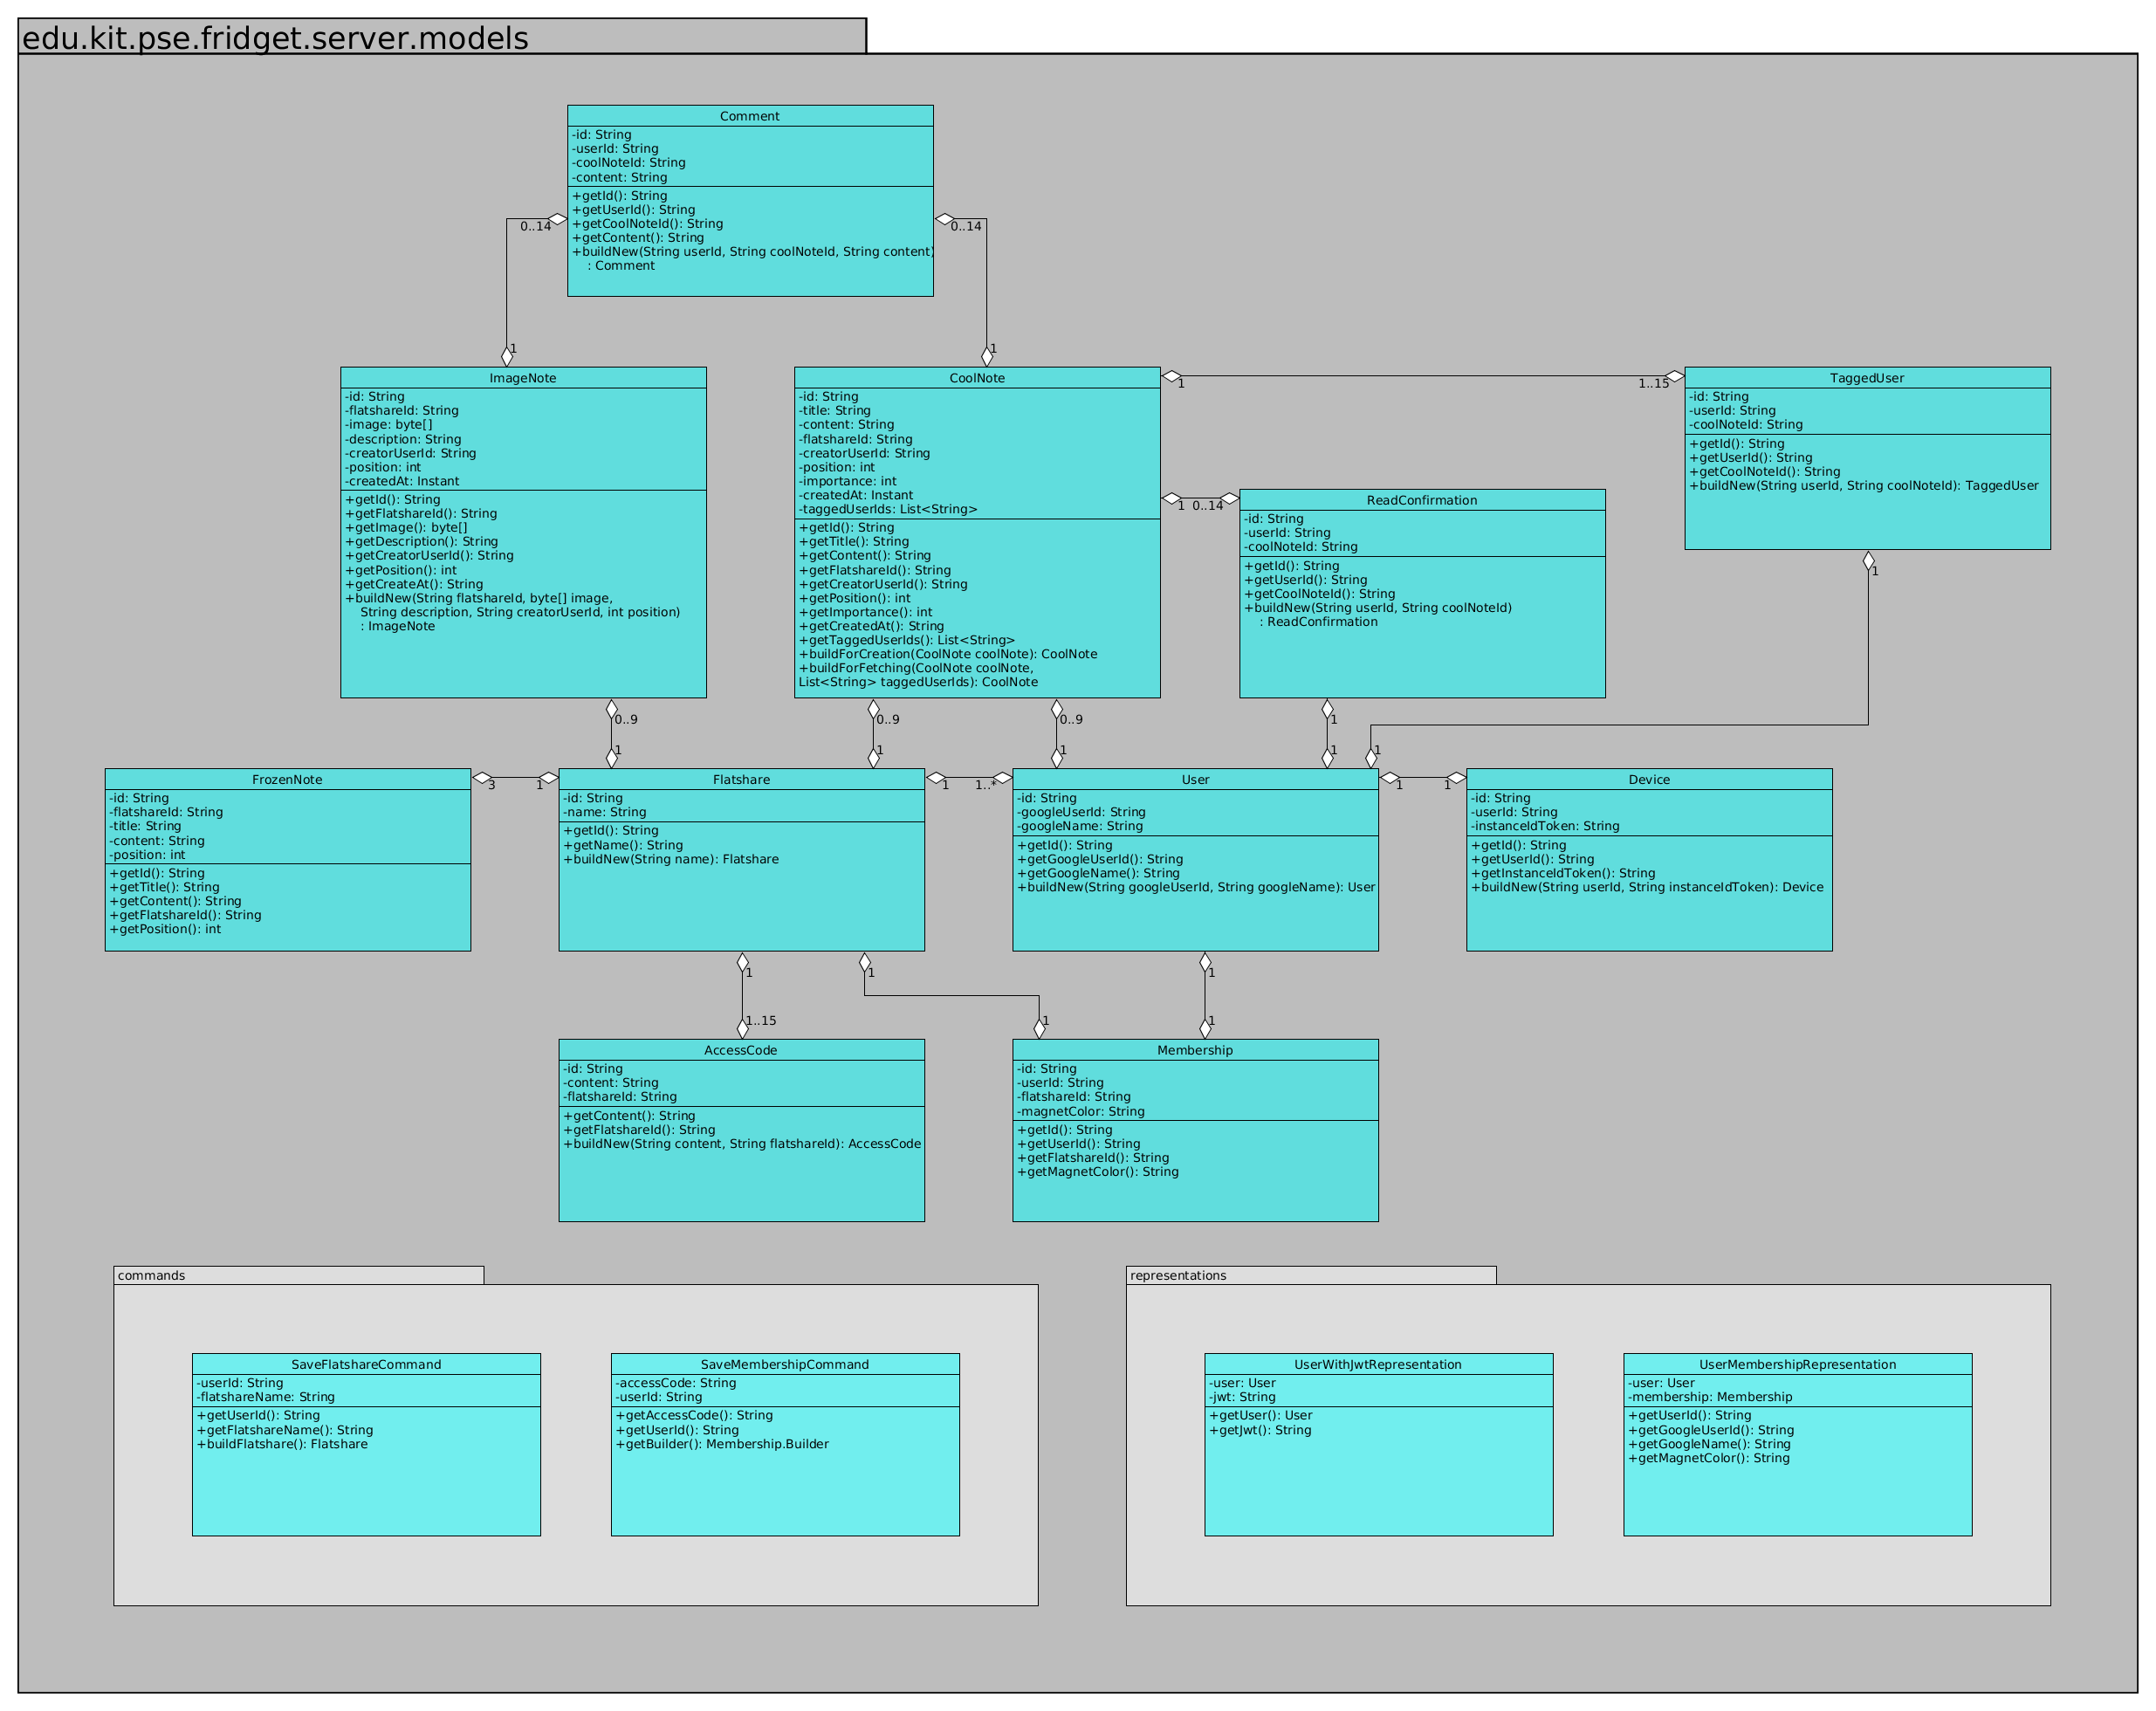
\includegraphics[scale = .20]{server-models.png}
	       \caption{Klassen des Models(Server)}
	      \end{figure}
     \subsubsection{\texttt{Class AccessCode}}
     \textbf{Beschreibung} \\
     \textit{Model für Zugangscode}
     \paragraph*{Methoden}
     \begin{itemize}
     	\item{\texttt{public String getId()}}
     	
     	\textit{Getter für Zugangscode-ID}
     	
     	\textbf{Rückgabewert}
     	\begin{itemize}
     		\item\textit{Zugangscode-ID}
     	\end{itemize}
     
     \item{\texttt{public String getContent()}}
     	
     	\textit{Getter für Inhalt vom Zugangscode}
     	
     	\textbf{Rückgabewert}
     	\begin{itemize}
     		\item\textit{Zugangscode-Inhalt}
     	\end{itemize}
     
     \item{\texttt{public String getFlatshareId()}}
     	
     	\textit{Getter für WG-ID}
     	
     	\textbf{Rückgabewert}
     	\begin{itemize}
     		\item\textit{WG-ID}
     	\end{itemize}
     
     \item{\texttt{public AccessCode buildNew(String content, String flatshareId)}}
     	
     	\textit{Baut Zugangscode mit zufälliger UUID.}
     	
     	\textbf{Parameter}
     	\begin{itemize}
     		\item\texttt{content}\\
     		\textit{Inhalt vom Zugangscode} 
     		\item\texttt{flatshareId}\\
     		\textit{ID von der WG, zu der mit dem Zugangscode beigetreten werden kann} 
     	\end{itemize}
     	
     	\textbf{Rückgabewert}
     	\begin{itemize}
     		\item\textit{Gebauter Zugangscode mit zufälliger UUID}
     	\end{itemize}
     \end{itemize}
 
     \subsubsection{\texttt{Class Comment}}
     \textbf{Beschreibung} \\
     \textit{Model für Kommentar}
     \paragraph*{Methoden}
     \begin{itemize}
     	\item{\texttt{public String getId()}}
     	
     	\textit{Getter für Kommentar-ID}
     	
     	\textbf{Rückgabewert}
     	\begin{itemize}
     		\item\textit{Kommentar-ID}
     	\end{itemize}
     
     \item{\texttt{public String getUserId()}}
     	
     	\textit{Getter für ID von dem Benutzer, der den Kommentar geschrieben hat}
     	
     	\textbf{Rückgabewert}
     	\begin{itemize}
     		\item\textit{Benutzer-ID}
     	\end{itemize}
     
     \item{\texttt{public String getCoolNoteId()}}
     	
     	\textit{Getter für ID von der Cool Note, zu der der Kommentar gehört}
     	
     	\textbf{Rückgabewert}
     	\begin{itemize}
     		\item\textit{CoolNote-ID}
     	\end{itemize}
     
     \item{\texttt{public String getContent()}}
     	
     	\textit{Getter für Inhalt vom Kommentar}
     	
     	\textbf{Rückgabewert}
     	\begin{itemize}
     		\item\textit{Kommentar-Inhalt}
     	\end{itemize}
     
     \item{\texttt{public Comment buildNew(String userId, String coolNoteId, String content)}}
     	
     	\textit{Baut Kommentar mit zufälliger UUID.}
     	
     	\textbf{Parameter}
     	\begin{itemize}
     		\item\texttt{userId}\\
     		\textit{ID von dem Benutzer, der den Kommentar geschrieben hat} 
     		\item\texttt{coolNoteId}\\
     		\textit{ID von der Cool Note, zu der der Kommentar gehört} 
     		\item\texttt{content}\\
     		\textit{Inhalt vom Kommentar}
     	\end{itemize}
     	
     	\textbf{Rückgabewert}
     	\begin{itemize}
     		\item\textit{Gebauter Kommentar mit zufälliger UUID}
     	\end{itemize}
     \end{itemize}
 
     \subsubsection{\texttt{Class CoolNote}}
     \textbf{Beschreibung} \\
     \textit{Model für Cool Note}
     \paragraph*{Methoden}
     \begin{itemize}
     	\item{\texttt{public String getId()}}
     	
     	\textit{Getter für Cool-Note-ID}
     	
     	\textbf{Rückgabewert}
     	\begin{itemize}
     		\item\textit{Cool-Note-ID}
     	\end{itemize}
     
     \item{\texttt{public String getTitle()}}
     	
     	\textit{Getter für Überschrift von der Cool Note}
     	
     	\textbf{Rückgabewert}
     	\begin{itemize}
     		\item\textit{Cool-Note-Überschrift}
     	\end{itemize}
     
     \item{\texttt{public String getContent()}}
     	
     	\textit{Getter für Inhalt von der Cool Note}
     	
     	\textbf{Rückgabewert}
     	\begin{itemize}
     		\item\textit{Cool-Note-Inhalt}
     	\end{itemize}
     
     \item{\texttt{public String getFlatshareId()}}
     	
     	\textit{Getter für ID von der WG, zu der diese Cool Note gehört}
     	
     	\textbf{Rückgabewert}
     	\begin{itemize}
     		\item\textit{WG-ID}
     	\end{itemize}
     
     \item{\texttt{public String getCreatorUserId()}}
     	
     	\textit{Getter für ID vom Benutzer, der die Cool Note erstellt hat}
     	
     	\textbf{Rückgabewert}
     	\begin{itemize}
     		\item\textit{Benutzer-ID}
     	\end{itemize}
     
     \item{\texttt{public int getPosition()}}
     	
     	\textit{Getter für Position der Cool Note auf der Pinnwand}
     	
     	\textbf{Rückgabewert}
     	\begin{itemize}
     		\item\textit{Position der Cool Note}
     	\end{itemize}
     
     \item{\texttt{public int getImportance()}}
     	
     	\textit{Getter für Wichtigkeit der Cool Note}
     	
     	\textbf{Rückgabewert}
     	\begin{itemize}
     		\item\textit{Wichtigkeit der Cool Note}
     	\end{itemize}
     
     \item{\texttt{public Instant getCreatedAt()}}
     	
     	\textit{Getter für Erstelldatum der Cool Note}
     	
     	\textbf{Rückgabewert}
     	\begin{itemize}
     		\item\textit{Erstelldatum der Cool Note}
     	\end{itemize}
     
     \item{\texttt{public List<String> getTaggedUserIds()}}
     	
     	\textit{Getter für IDs von den in dieser Cool Note getaggten Benutzern}
     	
     	\textbf{Rückgabewert}
     	\begin{itemize}
     		\item\textit{Liste von IDs von den getaggten Benutzern}
     	\end{itemize}
     \end{itemize}
 
     \subsubsection{\texttt{Class Device}}
     \textbf{Beschreibung} \\
     \textit{Model für Gerät}
     \paragraph*{Methoden}
     \begin{itemize}
     	\item{\texttt{public String getId()}}
     	
     	\textit{Getter für ID vom Gerät}
     	
     	\textbf{Rückgabewert}
     	\begin{itemize}
     		\item\textit{Gerät-ID}
     	\end{itemize}
     
     \item{\texttt{public String getUserId()}}
     	
     	\textit{Getter für ID vom Benutzer, der die App auf dem Gerät benutzt}
     	
     	\textbf{Rückgabewert}
     	\begin{itemize}
     		\item\textit{Benutzer-ID}
     	\end{itemize}
     
     \item{\texttt{public String getInstanceIdToken()}}
     	
     	\textit{Getter für ID von der App-Instanz auf dem Gerät}
     	
     	\textbf{Rückgabewert}
     	\begin{itemize}
     		\item\textit{Instanz-ID}
     	\end{itemize}
     
     \item{\texttt{public Device buildNew(String userId, String instanceIdToken)}}
     	
     	\textit{Baut Gerät mit zufälliger UUID.}
     	
     	\textbf{Parameter}
     	\begin{itemize}
     		\item\texttt{userId}\\
     		\textit{Benutzer-ID} 
     		\item\texttt{instanceIdToken}\\
     		\textit{Instanz-ID-Token}
     	\end{itemize}
     	
     	\textbf{Rückgabewert}
     	\begin{itemize}
     		\item\textit{Gebautes Gerät mit zufälliger UUID}
     	\end{itemize}
     \end{itemize}
 
     \subsubsection{\texttt{Class Flatshare}}
     \textbf{Beschreibung} \\
     \textit{Model für WG}
     \paragraph*{Methoden}
     \begin{itemize}
     	\item{\texttt{public String getId()}}
     	
     	\textit{Getter für WG-ID}
     	
     	\textbf{Rückgabewert}
     	\begin{itemize}
     		\item\textit{WG-ID}
     	\end{itemize}
     
     \item{\texttt{public String getName()}}
     	
     	\textit{Getter für WG-Name}
     	
     	\textbf{Rückgabewert}
     	\begin{itemize}
     		\item\textit{WG-Name}
     	\end{itemize}
     
     \item{\texttt{public Flatshare buildNew(String name)}}
     	
     	\textit{Baut WG mit zufälliger UUID.}
     	
     	\textbf{Parameter}
     	\begin{itemize}
     		\item\texttt{name}\\
     		\textit{Name von der WG}
     	\end{itemize}
     
     	\textbf{Rückgabewert}
     	\begin{itemize}
     		\item\textit{Gebaute WG mit zufälliger UUID}
     	\end{itemize}
     \end{itemize}
 
     \subsubsection{\texttt{Class FrozenNote}}
     \textbf{Beschreibung} \\
     \textit{Model für Frozen Note}
     \paragraph*{Methoden}
     \begin{itemize}
     	\item{\texttt{public String getId()}}
     	
     	\textit{Getter für Frozen-Note-ID}
     	
     	\textbf{Rückgabewert}
     	\begin{itemize}
     		\item\textit{Frozen-Note-ID}
     	\end{itemize}
     
     \item{\texttt{public String getTitle()}}
     	
     	\textit{Getter für Überschrift von der Frozen Note}
     	
     	\textbf{Rückgabewert}
     	\begin{itemize}
     		\item\textit{Frozen-Note-Überschrift}
     	\end{itemize}
     
     \item{\texttt{public String getContent()}}
     	
     	\textit{Getter für Inhalt von der Frozen Note}
     	
     	\textbf{Rückgabewert}
     	\begin{itemize}
     		\item\textit{Frozen-Note-Inhalt}
     	\end{itemize}
     
     \item{\texttt{public String getFlatshareId()}}
     	
     	\textit{Getter für ID von der WG, zu der diese Frozen Note gehört}
     	
     	\textbf{Rückgabewert}
     	\begin{itemize}
     		\item\textit{WG-ID}
     	\end{itemize}
     
     \item{\texttt{public int getPosition()}}
     	
     	\textit{Getter für Position der Frozen Note auf der Pinnwand}
     	
     	\textbf{Rückgabewert}
     	\begin{itemize}
     		\item\textit{Position der Frozen Note}
     	\end{itemize}
     \end{itemize}
     \subsubsection{\texttt{Class ImageNote}}
     \textbf{Beschreibung} \\
     \textit{Model für Image-Cool-Note}
     \paragraph*{Methoden}
     \begin{itemize}
     	\item{\texttt{public String getId()}}
     	
     	\textit{Getter für ImageNote-ID}
     	
     	\textbf{Rückgabewert}
     	\begin{itemize}
     		\item\textit{Image-Note-ID}
     	\end{itemize}
     
     \item{\texttt{public String getFlatshareId()}}
     	
     	\textit{Getter für ID von der WG, zu der diese Image-Cool-Note gehört}
     	
     	\textbf{Rückgabewert}
     	\begin{itemize}
     		\item\textit{WG-ID}
     	\end{itemize}
     
     \item{\texttt{public byte[] getImage()}}
     	
     	\textit{Getter für Bild in der Image-Cool-Note}
     	
     	\textbf{Rückgabewert}
     	\begin{itemize}
     		\item\textit{Bild}
     	\end{itemize}
     
     \item{\texttt{public String getDescription()}}
     	
     	\textit{Getter für Beschreibung der Image-Cool-Note}
     	
     	\textbf{Rückgabewert}
     	\begin{itemize}
     		\item\textit{Beschreibung der Image-Cool-Note}
     	\end{itemize}
     
     \item{\texttt{public String getCreatorUserId()}}
     	
     	\textit{Getter für ID vom Benutzer, der die Image-Cool-Note erstellt hat}
     	
     	\textbf{Rückgabewert}
     	\begin{itemize}
     		\item\textit{Benutzer-ID}
     	\end{itemize}
     
     \item{\texttt{public int getPosition()}}
     	
     	\textit{Getter für Position der Image Cool Note auf der Pinnwand}
     	
     	\textbf{Rückgabewert}
     	\begin{itemize}
     		\item\textit{Position der Image-Cool-Note}
     	\end{itemize}
     
     \item{\texttt{public String getCreateAt()}}
     	
     	\textit{Getter für Erstelldatum der Image-Cool-Note}
     	
     	\textbf{Rückgabewert}
     	\begin{itemize}
     		\item\textit{Erstelldatum der Image-Cool-Note}
     	\end{itemize}
     
     \item{\texttt{public ImageNote buildNew(String flatshareId, byte[] image, String description, String creatorUserId, int position)}}
     	
     	\textit{Baut Image Cool Note mit zufälliger UUID und aktuellem Datum.}
     	
     	\textbf{Parameter}
     	\begin{itemize}
     		\item\texttt{flatshareId}\\
     		\textit{ID von der WG, zu der diese Image-Cool-Note gehört}
     		\item\texttt{image}\\
     		\textit{Bild in der Image-Cool-Note}
     		\item\texttt{description}\\
     		\textit{Beschreibung der Image-Cool-Note}
     		\item\texttt{creatorUserId}\\
     		\textit{ID vom Benutzer, der die Image-Cool-Note erstellt hat}
     		\item\texttt{position}\\
     		\textit{Position der Image-Cool-Note auf der Pinnwand}
     	\end{itemize}
     
     	\textbf{Rückgabewert}
     	\begin{itemize}
     		\item\textit{Gebaute Image-Cool-Note mit zufälliger UUID und aktuellem Datum}
     	\end{itemize}
     \end{itemize}
     \subsubsection{\texttt{Class Membership}}
     \textbf{Beschreibung} \\
     \textit{Model für Mitgliedschaft}
     \paragraph*{Methoden}
     \begin{itemize}
     	\item{\texttt{public String getId()}}
     	
     	\textit{Getter für ID von der Mitgliedschaft}
     	
     	\textbf{Rückgabewert}
     	\begin{itemize}
     		\item\textit{Mitgliedschafts-ID}
     	\end{itemize}
     
     \item{\texttt{public String getUserId()}}
     	
     	\textit{Getter für ID vom Mitglied}
     	
     	\textbf{Rückgabewert}
     	\begin{itemize}
     		\item\textit{Benutzer-ID}
     	\end{itemize}
     
     \item{\texttt{public String getFlatshareId()}}
     	
     	\textit{Getter für WG-ID}
     	
     	\textbf{Rückgabewert}
     	\begin{itemize}
     		\item\textit{WG-ID}
     	\end{itemize}
     
     \item{\texttt{public String getMagnetColor()}}
     	
     	\textit{Getter für Magnetfarbe, die dem Mitglied in der WG zugeteilt wird}
     	
     	\textbf{Rückgabewert} 
     	\begin{itemize}
     		\item\textit{Magenetfarbe}
     	\end{itemize}
     \end{itemize}
     \subsubsection{\texttt{Class ReadConfirmation}}
     \textbf{Beschreibung} \\
     \textit{Model für Lesebestätigung}
     \paragraph*{Methoden}
     \begin{itemize}
     	\item{\texttt{public String getId()}}
     	
     	\textit{Getter für Lesebestätigung-ID}
     	
     	\textbf{Rückgabewert}
     	\begin{itemize}
     		\item\textit{Lesebestätigungs-ID}
     	\end{itemize}
     
     \item{\texttt{public String getUserId()}}
     	
     	\textit{Getter für ID vom Benutzer, der die Cool Note gelesen hat}
     	
     	\textbf{Rückgabewert}
     	\begin{itemize}
     		\item\textit{Benutzer-ID}
     	\end{itemize}
     
     \item{\texttt{public String getCoolNoteId()}}
     	
     	\textit{Getter für ID vom Cool Note, die gelesen wurde}
     	
     	\textbf{Rückgabewert}
     	\begin{itemize}
     		\item\textit{Cool-Note-ID}
     	\end{itemize}
     
     \item{\texttt{public ReadConfirmation buildNew(String userId, String coolNoteId)}}
     	
     	\textit{Baut Lesebestätigung.}
     	
     	\textbf{Parameter}
     	\begin{itemize}
     		\item\texttt{userId}\\
     		\textit{ID vom Benutzer, der die Cool Note gelesen hat}
     		\item\texttt{coolNoteId}\\
     		\textit{ID von der Cool Note, die gelesen wurde}
     	\end{itemize}
     
     	\textbf{Rückgabewert}
     	\begin{itemize}
     		\item\textit{Gebaute Lesebestätigung}
     	\end{itemize}
     \end{itemize}
     \subsubsection{\texttt{Class TaggedUser}}
     \textbf{Beschreibung} \\
     \textit{Model für getaggte Mitglieder}
     \paragraph*{Methoden}
     \begin{itemize}
     	\item{\texttt{public String getId()}}
     	
     	\textit{Getter für ID vom getaggten Mitglied}
     	
     	\textbf{Rückgabewert}
     	\begin{itemize}
     		\item\textit{ID vom getaggten Mitglied}
     	\end{itemize}
     
     \item{\texttt{public String getUserId()}}
     	
     	\textit{Getter für ID vom Benutzer, der getaggt wurde}
     	
     	\textbf{Rückgabewert}
     	\begin{itemize}
     		\item\textit{Benutzer-ID}
     	\end{itemize}
     
     \item{\texttt{public String getCoolNoteId()}}
     	
     	\textit{Getter für ID von der Cool Note, in der der Benutzer getaggt wurde}
     	
     	\textbf{Rückgabewert}
     	\begin{itemize}
     		\item\textit{Cool-Note-ID}
     	\end{itemize}
     
     \item{\texttt{public TaggedUser buildNew(String userId, String coolNoteId)}}
     	
     	\textit{Baut getaggtes Mitglied.}
     	
     	\textbf{Parameter}
     	\begin{itemize}
     		\item\texttt{userId}\\
     		\textit{ID vom Benutzer, der getaggt wurde}
     		\item\texttt{coolNoteId}\\
     		\textit{ID von der Cool Note, in der der Benutzer getaggt wurde}
     	\end{itemize}
     
     	\textbf{Rückgabewert}
     	\begin{itemize}
     		\item\textit{Gebautes getaggtes Mitglied}
     	\end{itemize}
     \end{itemize}
     \subsubsection{\texttt{Class User}}
     \textbf{Beschreibung} \\
     \textit{Model für Benutzer}
     \paragraph*{Methoden}
     \begin{itemize}
     	\item{\texttt{public String getId()}}
     	
     	\textit{Getter für Benutzer-ID}
     	
     	\textbf{Rückgabewert} 
     	\begin{itemize}
     		\item\textit{Benutzer-ID}
     	\end{itemize}
     
     \item{\texttt{public String getGoogleUserId()}}
     	
     	\textit{Getter für Google-ID vom Benutzer}
     	
     	\textbf{Rückgabewert}
     	\begin{itemize}
     		\item\textit{Google-ID}
     	\end{itemize}
     
     \item{\texttt{public String getGoogleName()}}
     	
     	\textit{Getter für Google-Name vom Benutzer}
     	
     	\textbf{Rückgabewert}
     	\begin{itemize}
     		\item\textit{Google-Name}
     	\end{itemize}
     
     \item{\texttt{public User buildNew(String googleUserId, String googleName)}}
     	
     	\textit{Baut Benutzer mit zufälliger UUID.}
     	
     	\textbf{Parameter}
     	\begin{itemize}
     		\item\texttt{googleUserId}\\
     		\textit{Google-ID vom Benutzer}
     		\item\texttt{googleName}\\
     		\textit{Google-Name vom Benutzer}
     	\end{itemize}
     	
     	\textbf{Rückgabewert}
     	\begin{itemize}
     		\item\textit{Gebauter Benutzer mit zufälliger UUID}
     	\end{itemize}
     \end{itemize}
     \subsection{Package edu.kit.pse.fridget.server.models.commands}
     \subsubsection{\texttt{Class SaveFlatshareCommand}}
     \textbf{Beschreibung} \\
     \textit{Model für das Speichern der WG}
     \paragraph*{Konstruktor}\mbox{} \\
     \texttt{public SaveFlatshareCommand(String userId, String flatshareName)} 
     \paragraph*{Methoden}
     \begin{itemize}
     	\item{\texttt{public String getUserId()}}
     	
     	\textit{Getter für ID vom Benutzer, der die WG erstellt hat}
     	
     	\textbf{Rückgabewert}
     	\begin{itemize}
     		\item\textit{Benutzer-ID}
     	\end{itemize}
     
     \item{\texttt{public String getFlatshareName()}}
     	
     	\textit{Getter für Name von der WG}
     	
     	\textbf{Rückgabewert}
     	\begin{itemize}
     		\item\textit{WG-Name}
     	\end{itemize}
     
     \item{\texttt{public Flatshare buildFlatshare()}}
     	
     	\textit{Baut eine WG-Instanz.}
     	
     	\textbf{Rückgabewert}
     	\begin{itemize}
     		\item\textit{WG}
     	\end{itemize}
     \end{itemize}
 
     \subsubsection{\texttt{Class SaveMembershipCommand}}
     \textbf{Beschreibung} \\
     \textit{Model für das Speichern der Mitgliedschaft}
     \paragraph*{Konstruktor}\mbox{} \\
     \texttt{public SaveMembershipCommand(String accessCode, String userId)}
     \paragraph*{Methoden}
     \begin{itemize}
     	\item{\texttt{public String getAccessCode()}}
     	
     	\textit{Getter für Zugangscode}
     	
     	\textbf{Rückgabewert}
     	\begin{itemize}
     		\item\textit{Zugangscode}
     	\end{itemize}
     
     \item{\texttt{public String getUserId()}}
     	
     	\textit{ID vom Benutzer, der der WG beitritt}
     	
     	\textbf{Rückgabewert}
     	\begin{itemize}
     		\item\textit{Benutzer-ID}
     	\end{itemize}
     
     \item{\texttt{public Membership.Builder getBuilder()}}
     	
     	\textit{Getter für Builder von Mitgliedschaft}
     	
     	\textbf{Rückgabewert}
     	\begin{itemize}
     		\item\textit{Builder von Mitgliedschaft}
     	\end{itemize}
     \end{itemize}
 
     \subsection{Package edu.kit.pse.fridget.server.models.representations}
     \subsubsection{\texttt{Class UserMembershipRepresentation}}
     \textbf{Beschreibung} \\
     \textit{Model für Benutzer mit Mitgliedschaft-Info}
     \paragraph*{Konstruktor}\mbox{} \\
     \texttt{public UserMembershipRepresentation(User user, Membership membership)}
     \paragraph*{Methoden}
     \begin{itemize}
     	\item{\texttt{public String getUserId()}}
     	
     	\textit{Getter für ID vom Benutzer}
     	
     	\textbf{Rückgabewert}
     	\begin{itemize}
     		\item\textit{Benutzer-ID}
     	\end{itemize}
     
     \item{\texttt{public String getGoogleUserId()}}
     	
     	\textit{Getter für Google-ID vom Benutzer}
     	
     	\textbf{Rückgabewert}
     	\begin{itemize}
     		\item\textit{Google-User-ID}
     	\end{itemize}
     
     \item{\texttt{public String getGoogleName()}}
     	
     	\textit{Getter für Google-Name von Benutzer}
     	
     	\textbf{Rückgabewert}
     	\begin{itemize}
     		\item\textit{Google-Name}
     	\end{itemize}
     
     \item{\texttt{public String getMagnetColor()}}
     	
     	\textit{Getter für Magnetfarbe, die dem Benutzer zugeteilt wurde}
     	
     	\textbf{Rückgabewert}
     	\begin{itemize}
     		\item\textit{Benutzer}
     	\end{itemize}
     \end{itemize}
 
     \subsubsection{\texttt{Class UserWithJwtRepresentation}}
     \textbf{Beschreibung} \\
     \textit{Model für Benutzer mit JWT (JSON Web Token)}
     \paragraph*{Konstruktor}\mbox{} \\
     \texttt{public UserWithJwtRepresentation(User user, String jwt)}
     \paragraph*{Methoden}
     \begin{itemize}
     	\item{\texttt{public User getUser()}}
     	
     	\textit{Getter für Benutzer}
     	
     	\textbf{Rückgabewert}
     	\begin{itemize}
     		\item\textit{Benutzer}
     	\end{itemize}
     
     \item{\texttt{public String getJwt()}}
     	
     	\textit{Getter für JWT}
     	
     	\textbf{Rückgabewert}
     	\begin{itemize}
     		\item\textit{JWT}
     	\end{itemize}
     \end{itemize}
 
     \subsection{Package edu.kit.pse.fridget.server.repositories}
     \begin{figure}[H]
	       \centering
	       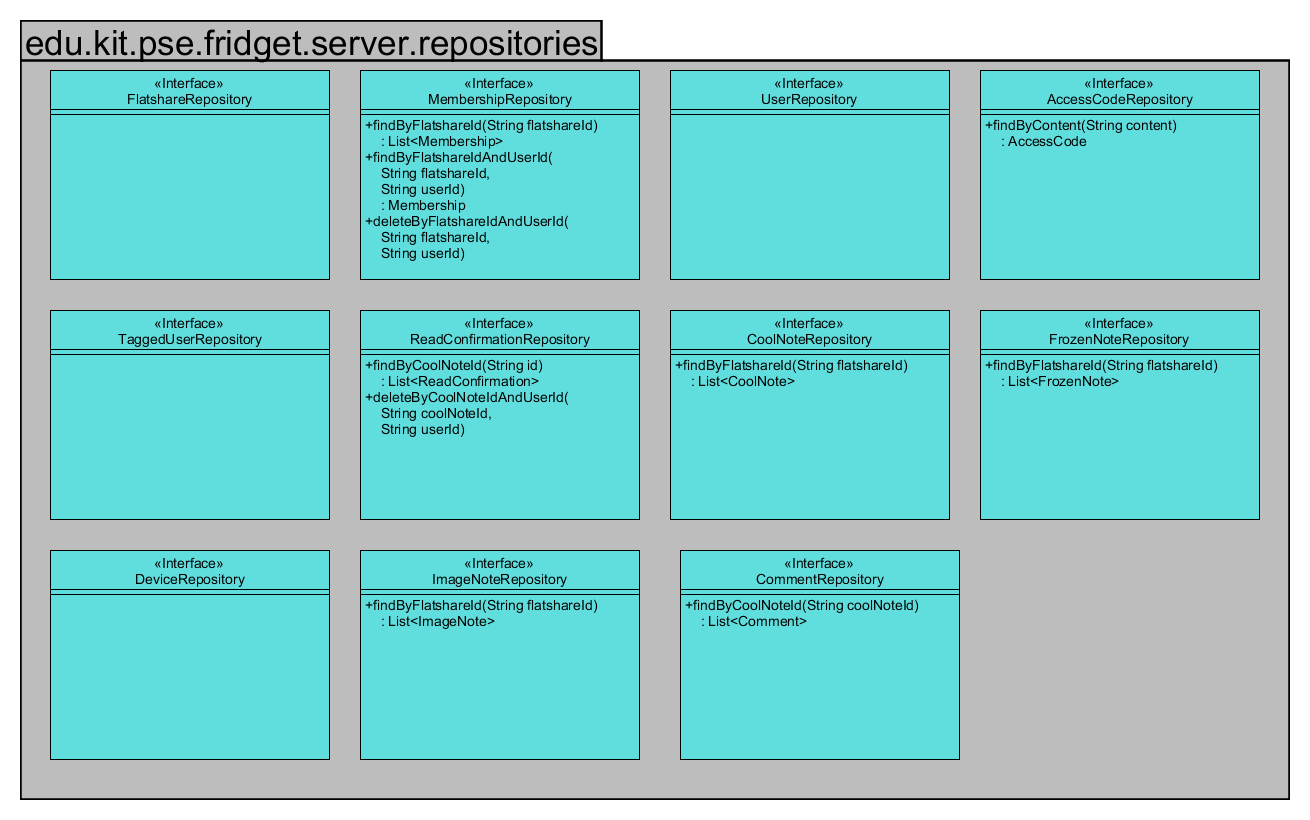
\includegraphics[scale = .35]{server-repositories.png}
	       \caption{Klassen des Repositories}
	      \end{figure}
     \subsubsection{\texttt{Interface AccessCodeRepository extends JpaRepository<AccessCode,String>}}
     \textbf{Beschreibung} \\
     \textit{Repository für Zugangscode}
     \paragraph*{Methoden}
     \begin{itemize}
     	\item{\texttt{public AccessCode findByContent(String content)}}
     	
     	\textit{Findet einen Zugangscode über Inhalt.}
     	
     	\textbf{Parameter}
     	\begin{itemize}
     		\item\texttt{content}\\
     		\textit{Inhalt des Zugangscodes}
     	\end{itemize}
     	
     	\textbf{Rückgabewert}
     	\begin{itemize}
     		\item\textit{Gefundener Zugangscode}
     	\end{itemize}
     \end{itemize}
     \subsubsection{\texttt{Interface CommentRepository extends JpaRepository<Comment,String>}}
     \textbf{Beschreibung} \\
     \textit{Repository für Kommentar}
     \paragraph*{Methoden}
     \begin{itemize}
     	\item{\texttt{public List<Comment> findByCoolNoteId(String coolNoteId)}}
     	
     	\textit{Findet alle Kommentare über Cool-Note-ID}
     	
     	\textbf{Parameter}
     	\begin{itemize}
     		\item\texttt{coolNoteId}\\
     		\textit{Cool-Note-ID}
     	\end{itemize}
     	
     	\textbf{Rückgabewert}
     	\begin{itemize}
     		\item\textit{Liste von gefundenen Kommentaren}
     	\end{itemize}
     \end{itemize}
     \subsubsection{\texttt{Interface CoolNoteRepository extends JpaRepository<CoolNote,String>}}
     \textbf{Beschreibung} \\
     \textit{Repository für Cool Note}
     \paragraph*{Methoden}
     \begin{itemize}
     	\item{\texttt{public List<CoolNote> findByFlatshareId(String flatshareId)}}
     	
     	\textit{Findet alle Cool Notes über WG-ID}
     	
     	\textbf{Parameter}
     	\begin{itemize}
     		\item\texttt{flatshareId}\\
     		\textit{WG-ID}
     	\end{itemize}
     	
     	\textbf{Rückgabewert}
     	\begin{itemize}
     		\item\textit{Liste von gefundenen Cool Notes}
     	\end{itemize}
     \end{itemize}
 
     \subsubsection{\texttt{Interface DeviceRepository extends JpaRepository<Device,String>}}
     \textbf{Beschreibung} \\
     \textit{Repository für Geräte}
     \subsubsection{\texttt{Interface FlatshareRepository extends JpaRepository<Flatshare,String>}}
     \textbf{Beschreibung} \\
     \textit{Repository für WG}
     \subsubsection{\texttt{Interface FrozenNoteRepository extends JpaRepository<FrozenNote,String>}}
     \textbf{Beschreibung} \\
     \textit{Repository für Frozen Note}
     \paragraph*{Methoden}
     \begin{itemize}
     	\item{\texttt{public List<FrozenNote> findByFlatshareId(String flatshareId)}}
     	
     	\textit{Findet alle Frozen Notes über WG-ID}
     	
     	\textbf{Parameter}
     	\begin{itemize}
     		\item\texttt{flatshareId}\\
     		\textit{WG-ID}
     	\end{itemize}
     	
     	\textbf{Rückgabewert}
     	\begin{itemize}
     		\item\textit{Liste von gefundenen Frozen Notes}
     	\end{itemize}
     \end{itemize}
 
     \subsubsection{\texttt{Interface ImageNoteRepository extends JpaRepository<ImageNote,String>}}
     \textbf{Beschreibung} \\
     \textit{Repository für Image Cool Note}
     \paragraph*{Methoden}
     \begin{itemize}
     	\item{\texttt{public List<ImageNote> findByFlatshareId(String flatshareId)}}
     	
     	\textit{Findet alle Image Cool Notes über WG-ID}
     	
     	\textbf{Parameter} 
     	\begin{itemize}
     		\item\texttt{flatshareId}\\
     		\textit{WG-ID}
     	\end{itemize}
     	
     	\textbf{Rückgabewert}
     	\begin{itemize}
     		\item\textit{Liste von gefundenen Image Cool Notes}
     	\end{itemize}
     \end{itemize}
 
     \subsubsection{\texttt{Interface MembershipRepository extends JpaRepository<Membership,String>}}
     \textbf{Beschreibung} \\
     \textit{Repository für Mitgliedschaft}
     \paragraph*{Methoden}
     \begin{itemize}
     	\item{\texttt{public List<Membership> findByFlatshareId(String flatshareId)}}
     	
     	\textit{Findet alle Mitgliedschaften über WG-ID}
     	
     	\textbf{Parameter}
     	\begin{itemize}
     		\item\texttt{flatshareId}\\
     		\textit{WG-ID}
     	\end{itemize}
     	
     	\textbf{Rückgabewert}
     	\begin{itemize}
     		\item\textit{Liste von gefundenen Mitgliedschaften}
     	\end{itemize}
     
     \item{\texttt{public Membership findByFlatshareIdAndUserId(String flatshareId, String userId)}}
     	
     	\textit{Findet eine Mitgliedschaft über WG-ID und Benutzer-ID}
     	
     	\textbf{Parameter}
     	\begin{itemize}
     		\item\texttt{flatshareId}\\
     		\textit{WG-ID}
     		\item\texttt{userId}\\
     		\textit{Benutzer-ID}
     	\end{itemize}
     
     	\textbf{Rückgabewert}
     	\begin{itemize}
     		\item\textit{Gefundene Mitgliedschaft}
     	\end{itemize}
     
     \item{\texttt{public void deleteByFlatshareIdAndUserId(String flatshareId, String userId)}}
     	
     	\textit{Löscht eine Mitgiedschaft über WG-ID und Benutzer-ID}
     	
     	\textbf{Parameter}
     	\begin{itemize}
     		\item\texttt{flatshareId}\\
     		\textit{WG-ID}
     		\item\texttt{userId}\\
     		\textit{Benutzer-ID}
     	\end{itemize}
     \end{itemize}
     
     \subsubsection{\texttt{Interface ReadConfirmationRepository extends JpaRepository<ReadConfirmation,String>}}
     \textbf{Beschreibung} \\
     \textit{Repository für Lesebestätigung}
     \paragraph*{Methoden}
     \begin{itemize}
     	\item{\texttt{public List<ReadConfirmation> findByCoolNoteId(String id)}}
     	
     	\textit{Findet alle Lesebestätigungen über CoolNote-ID}
     	
     	\textbf{Parameter}
     	\begin{itemize}
     		\item\texttt{id}\\
     		\textit{Cool-Note-ID}
     	\end{itemize}
     	
     	\textbf{Rückgabewert}
     	\begin{itemize}
     		\item\textit{Liste von gefundenen Lesebestätigungen}
     	\end{itemize}
     
     \item{\texttt{public void deleteByCoolNoteIdAndUserId(String coolNoteId, String userId)}}
     	
     	\textit{Löscht eine Lesebestätigung über Cool-Note-ID und Benutzer-ID}
     	
     	\textbf{Parameter}
     	\begin{itemize}
     		\item\texttt{coolNoteId}\\
     		\textit{Cool-Note-ID}
     		\item\texttt{userId}\\
     		\textit{Benutzer-ID}
     	\end{itemize}
     \end{itemize}
     
     \subsubsection{\texttt{Interface TaggedUserRepository extends JpaRepository<TaggedUser,String>}}
     \textbf{Beschreibung} \\
     \textit{Repository für getaggte Mitglieder}
     \subsubsection{\texttt{Interface UserRepository extends JpaRepository<User,String>}}
     \textbf{Beschreibung} \\
     \textit{Repository für User Entity}
     \subsection{Package edu.kit.pse.fridget.server.services}
     \begin{figure}[H]
	       \centering
	       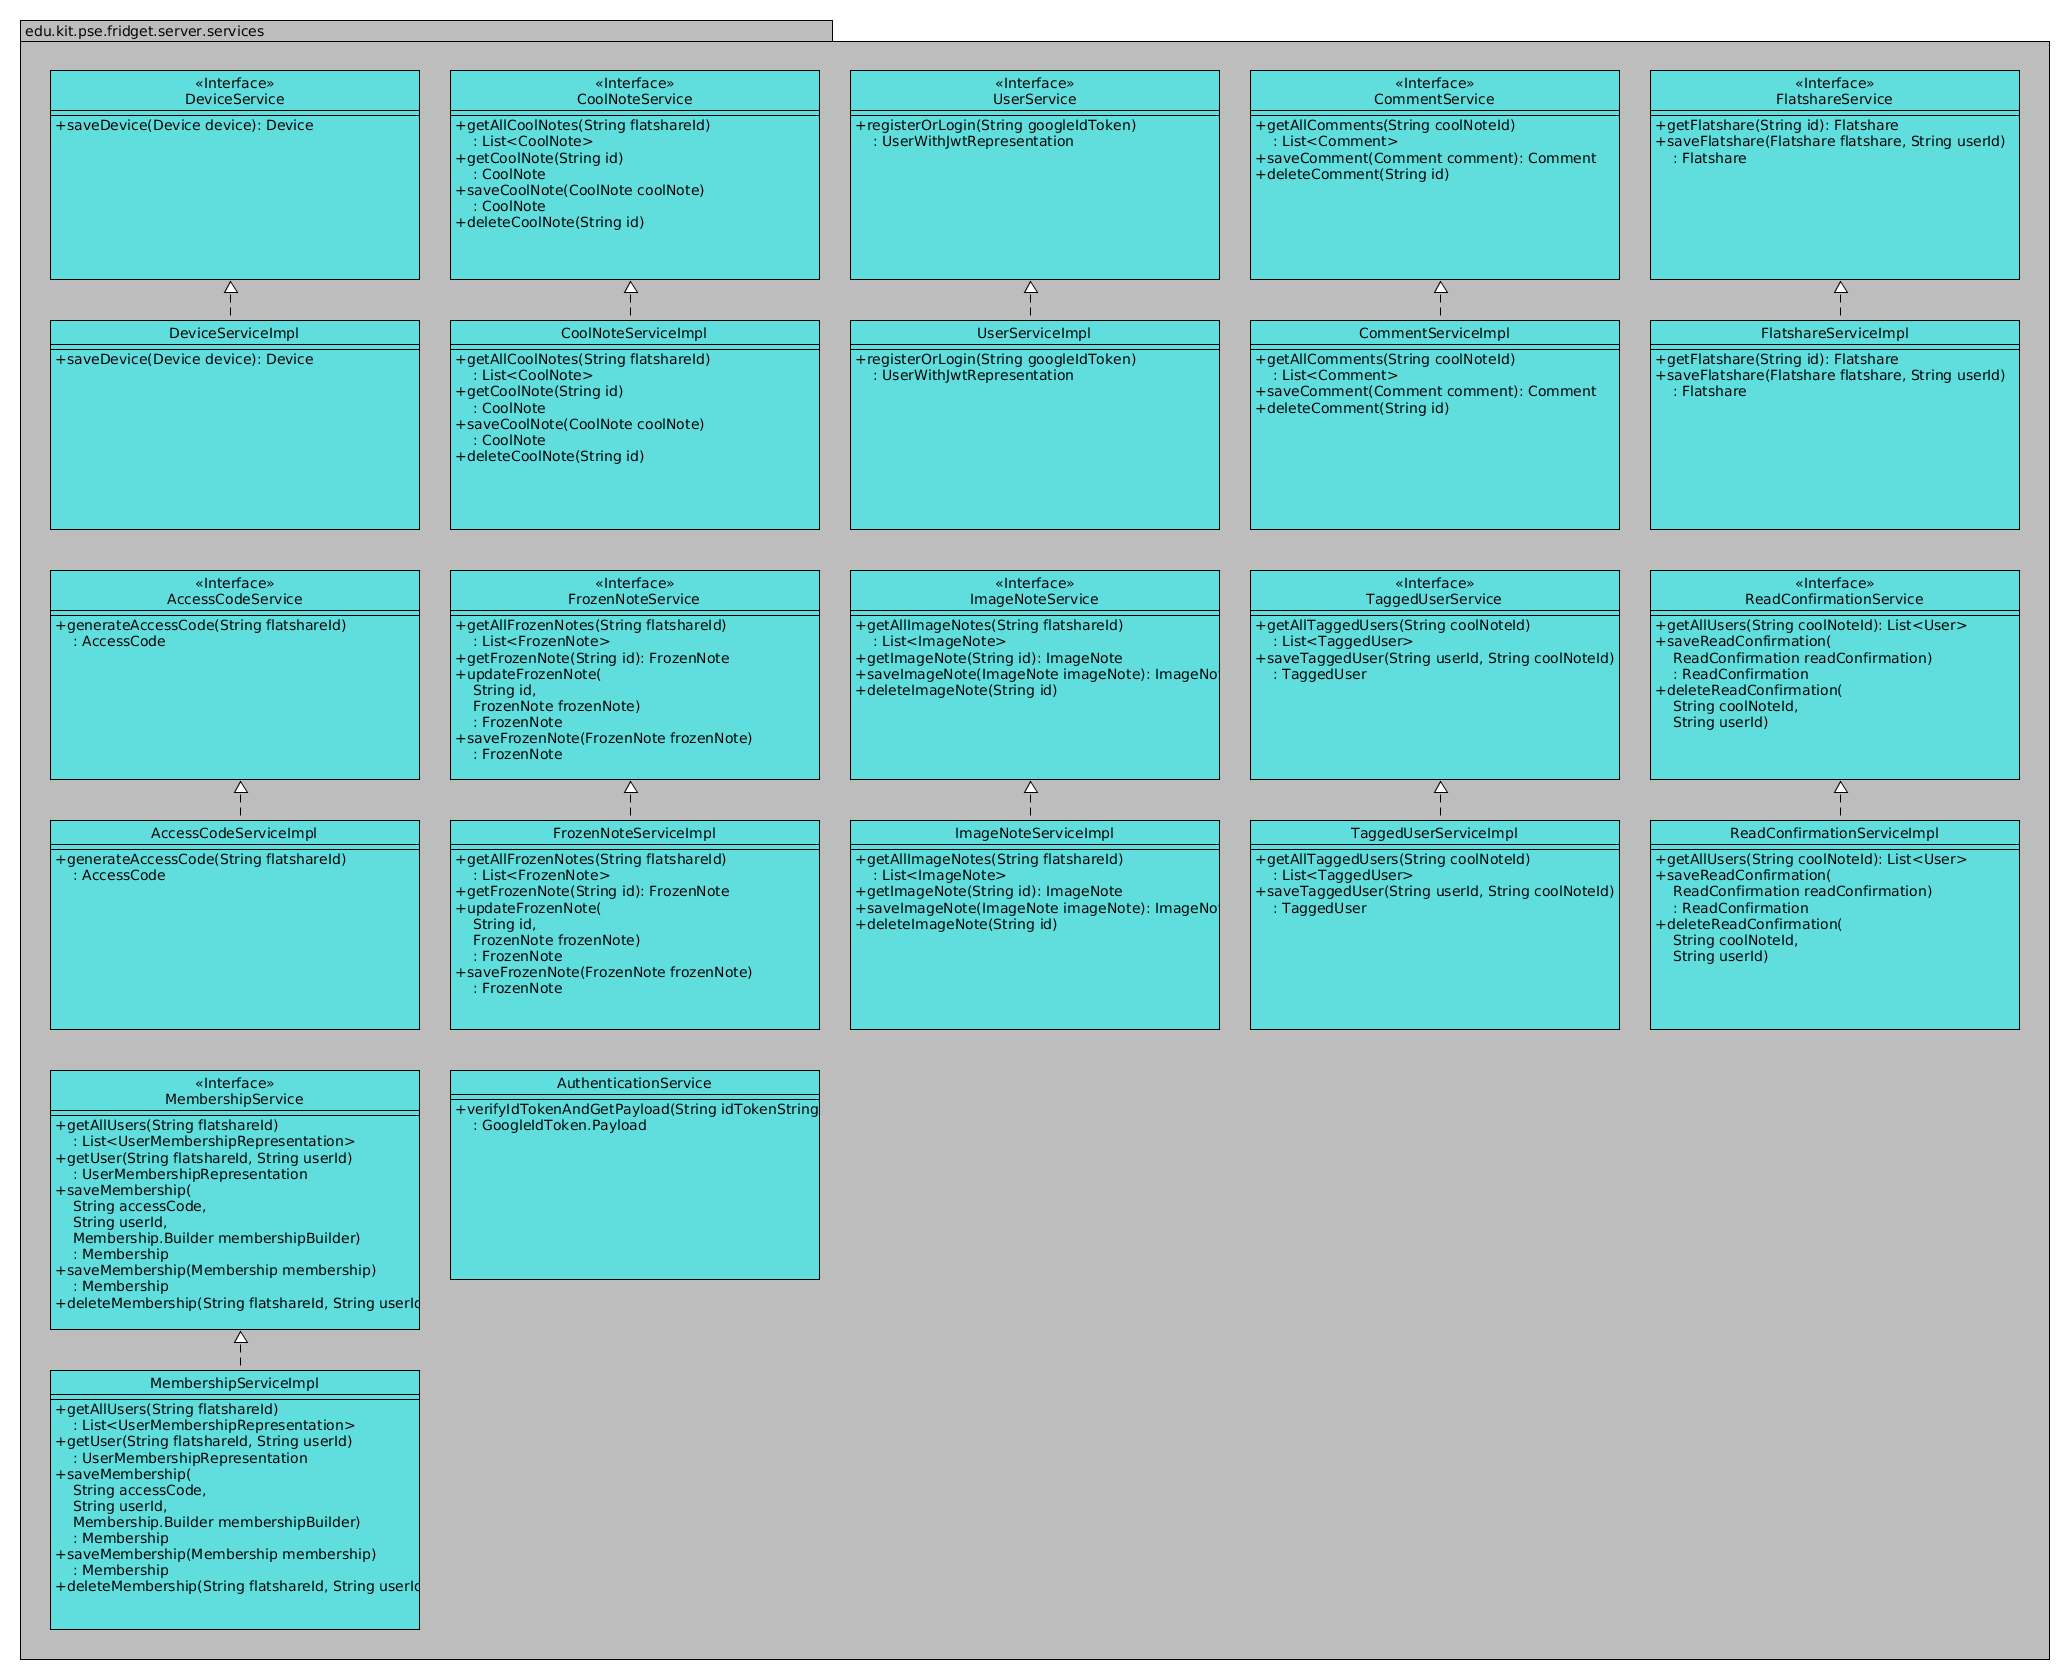
\includegraphics[scale = .22]{server-services.png}
	       \caption{Klassen des Services (Server)}
	      \end{figure}
     \subsubsection{\texttt{Interface AccessCodeService}}
     \textbf{Beschreibung} \\
     \textit{Interface von Service für Zugangscode}
     \paragraph*{Methoden}
     \begin{itemize}
     	\item{\texttt{public AccessCode generateAccessCode(String flatshareId)}}
     	
     	\textit{Generiert einen zufälligen und eindeutigen Zugangscode für eine WG.}
     	
     	\textbf{Parameter}
     	\begin{itemize}
     		\item\texttt{flatshareId}\\
     		\textit{WG-ID}
     	\end{itemize}
     
     	\textbf{Rückgabewert}
     	\begin{itemize}
     		\item\textit{Generierter Zugangscode}
     	\end{itemize}
     \end{itemize}
     \subsubsection{\texttt{Class AccessCodeServiceImpl implements AccessCodeService}}
     \textbf{Beschreibung} \\
     \textit{Service für Zugangscode}
     \paragraph*{Konstruktor}\mbox{} \\
     \texttt{public AccessCodeServiceImpl(AccessCodeRepository repository)}
     \subsubsection{\texttt{Class AuthenticationService}}
     \textbf{Beschreibung} \\
     \textit{Service für Authentifizierung}
     \paragraph*{Methoden}
     \begin{itemize}
     	\item{\texttt{public GoogleIdToken.Payload verifyIdTokenAndGetPayload(String idTokenString)}}
     	
     	\textit{Prüft den Google-ID-Token.}
     	
     	\textbf{Parameter}
     	\begin{itemize}
     		\item\texttt{idTokenString}\\
     		\textit{Google-ID-Token}
     	\end{itemize}
     	
     	\textbf{Rückgabewert}
     	\begin{itemize}
     		\item\textit{Payload von Google-ID-Token}
     	\end{itemize}
     \end{itemize}
 
     \subsubsection{\texttt{Interface CommentService}}
     \textbf{Beschreibung} \\
     \textit{Interface von Service für Kommentar}
     \paragraph*{Methoden}
     \begin{itemize}
     	\item{\texttt{public List<Comment> getAllComments(String coolNoteId)}}
     	
     	\textit{Findet alle Kommentare.}
     	
     	\textbf{Parameter}
     	\begin{itemize}
     		\item\texttt{coolNoteId}\\
     		\textit{Cool-Note-ID}
     	\end{itemize}
     	
     	\textbf{Rückgabewert}
     	\begin{itemize}
     		\item\textit{Liste von gefundenen Kommentaren}
     	\end{itemize}
     
     \item{\texttt{public Comment saveComment(Comment comment)}}
     	
     	\textit{Speichert einen Kommentar.}
     	
     	\textbf{Parameter}
     	\begin{itemize}
     		\item\texttt{comment}\\
     		\textit{Kommentar zum Speichern}
     	\end{itemize}
     	
     	\textbf{Rückgabewert}
     	\begin{itemize}
     		\item\textit{Gespeicherter Kommentar}
     	\end{itemize}
     
     \item{\texttt{public void deleteComment(String id)}}
     	
     	\textit{Löscht einen Kommentar.}
     	
     	\textbf{Parameter}
     	\begin{itemize}
     		\item\texttt{id}\\
     		\textit{Kommentar-ID}
     	\end{itemize}
     \end{itemize}
     \subsubsection{\texttt{Class CommentServiceImpl implements CommentService}}
     \textbf{Beschreibung} \\
     \textit{Service für Kommentar}
     \paragraph*{Konstruktor}\mbox{} \\
     \texttt{public CommentServiceImpl(CommentRepository repository)}
     \subsubsection{\texttt{Interface CoolNoteService}}
     \textbf{Beschreibung} \\
     \textit{Interface von Service für Cool Note}
     \paragraph*{Methoden}
     \begin{itemize}
     	\item{\texttt{public List<CoolNote> getAllCoolNotes(String flatshareId)}}
     	
     	\textit{Findet alle Cool Notes mit getaggten Benutzern in einer WG.}
     	
     	\textbf{Parameter}
     	\begin{itemize}
     		\item\texttt{flatshareId}\\
     		\textit{WG-ID}
     	\end{itemize}
     	
     	\textbf{Rückgabewert}
     	\begin{itemize}
     		\item\textit{Liste von gefundenen Cool Notes mit getaggten Benutzern}
     	\end{itemize}
     
     \item{\texttt{public CoolNote getCoolNote(String id)}}
     	
     	\textit{Findet eine Cool Note mit getaggten Benutzern.}
     	
     	\textbf{Parameter}
     	\begin{itemize}
     		\item\texttt{id}\\
     		\textit{Cool-Note-ID}
     	\end{itemize}
     
     	\textbf{Rückgabewert}
     	\begin{itemize}
     		\item\textit{Gefundene Cool Note mit getaggten Benutzern}
     	\end{itemize}
     
     \item{\texttt{public CoolNote saveCoolNote(CoolNote coolNote)}}
     	
     	\textit{Speichert eine Cool Note.}
     	
     	\textbf{Parameter}
     	\begin{itemize}
     		\item\texttt{coolNote}\\
     		\textit{Cool Note zum Speichern}
     	\end{itemize}
     	
     	\textbf{Rückgabewert}
     	\begin{itemize}
     		\item\textit{Gespeicherte Cool Note}
     	\end{itemize}
     
     \item{\texttt{public void deleteCoolNote(String id)}}
     	
     	\textit{Löscht eine Cool Note.}
     	
     	\textbf{Parameter}
     	\begin{itemize}
     		\item\texttt{id}\\
     		\textit{Cool-Note-ID}
     	\end{itemize}
     \end{itemize}
     
     \subsubsection{\texttt{Class CoolNoteServiceImpl implements CoolNoteService}}
     \textbf{Beschreibung} \\
     \textit{Service für Cool Note}
     \paragraph*{Konstruktor}\mbox{} \\
     \texttt{public CoolNoteServiceImpl(CoolNoteRepository coolNoteRepository, TaggedUserRepository taggedUserRepository)} \\
     \subsubsection{\texttt{Interface DeviceService}}
     \textbf{Beschreibung} \\
     \textit{Interface von Service für Gerät}
     \paragraph*{Methoden}
     \begin{itemize}
     	\item{\texttt{public Device saveDevice(Device device)}}
     	
     	\textit{Speichert ein neues Gerät.}
     	
     	\textbf{Parameter}
     	\begin{itemize}
     		\item\texttt{device}\\
     		\textit{Gerät zum Speichern}
     	\end{itemize}
     
     	\textbf{Rückgabewert}
     	\begin{itemize}
     		\item\textit{Gespeichertes Gerät}
     	\end{itemize}
     \end{itemize}
 
     \subsubsection{\texttt{Class DeviceServiceImpl implements DeviceService}}
     \textbf{Beschreibung} \\
     \textit{Service für Gerät}
     \paragraph*{Konstruktor}\mbox{} \\
     \texttt{public DeviceServiceImpl(DeviceRepository repository)}
     \subsubsection{\texttt{Interface FlatshareService}}
     \textbf{Beschreibung} \\
     \textit{Interface von Service für WG}
     \paragraph*{Methoden}
     \begin{itemize}
     	\item{\texttt{public Flatshare getFlatshare(String id)}}
     	
     	\textit{Findet eine WG.}
     	
     	\textbf{Parameter}
     	\begin{itemize}
     		\item\texttt{id}\\
     		\textit{WG-ID}
     	\end{itemize}
     	
     	\textbf{Rückgabewert}
     	\begin{itemize}
     		\item\textit{Gefundene WG}
     	\end{itemize}
     
     \item{\texttt{public Flatshare saveFlatshare(Flatshare flatshare, String userId)}}
     	
     	\textit{Speichert eine WG mit einem Namen.}
     	
     	\textbf{Parameter}
     	\begin{itemize}
     		\item\texttt{flatshare}\\
     		\textit{WG zum Speichern}
     		\item\texttt{userId}\\
     		\textit{Benutzer-ID}
     	\end{itemize}
     
     	\textbf{Rückgabewert}
     	\begin{itemize}
     		\item\textit{Gespeicherte WG}
     	\end{itemize}
     \end{itemize}
 
     \subsubsection{\texttt{Class FlatshareServiceImpl implements FlatshareService}}
     \textbf{Beschreibung} \\
     \textit{Service für WG}
     \paragraph*{Konstruktor}\mbox{} \\
     \texttt{public FlatshareServiceImpl(FlatshareRepository flatshareRepository, MembershipService membershipService, FrozenNoteService frozenNoteService)}
     \subsubsection{\texttt{Interface FrozenNoteService}}
     \textbf{Beschreibung} \\
     \textit{Interface von Service für Frozen Note}
     \paragraph*{Methoden}
     \begin{itemize}
     	\item{\texttt{public List<FrozenNote> getAllFrozenNotes(String flatshareId)}}
     	
     	\textit{Findet alle Frozen Notes in einer WG.}
     	
     	\textbf{Parameter}
     	\begin{itemize}
     		\item\texttt{flatshareId}\\
     		\textit{WG-ID}
     	\end{itemize}
     	
     	\textbf{Rückgabewert}
     	\begin{itemize}
     		\item\textit{Liste von gefundenen Frozen Notes}
     	\end{itemize}
     
     \item{\texttt{public FrozenNote getFrozenNote(String id)}}
     	
     	\textit{Findet eine Frozen Note.}
     	
     	\textbf{Parameter}
     	\begin{itemize}
     		\item\texttt{id}\\
     		\textit{Frozen-Note-ID}
     	\end{itemize}
     	
     	\textbf{Rückgabewert}
     	\begin{itemize}
     		\item\textit{Gefundene Frozen Note}
     	\end{itemize}
     
     \item{\texttt{public FrozenNote updateFrozenNote(String id, FrozenNote frozenNote)}}
     	
     	\textit{Updatet eine Frozen Note.}
     	
     	\textbf{Parameter}
     	\begin{itemize}
     		\item\texttt{id}\\
     		\textit{Frozen-Note-ID}
     		\item\texttt{frozenNote}\\
     		\textit{Frozen Note zum Updaten}
     	\end{itemize}
     
     	\textbf{Rückgabewert}
     	\begin{itemize}
     		\item\textit{Geupdatete Frozen Note}
     	\end{itemize}
     
     \item{\texttt{public FrozenNote saveFrozenNote(FrozenNote frozenNote)}}
     	
     	\textit{Speichert eine Frozen Note.}
     	
     	\textbf{Parameter}
     	\begin{itemize}
     		\item\texttt{frozenNote}\\
     		\textit{Frozen Note zum Speichern}
     	\end{itemize}
     
     	\textbf{Rückgabewert}
     	\begin{itemize}
     		\item\textit{Gespeicherte Frozen Note}
     	\end{itemize}
     \end{itemize}
     \subsubsection{\texttt{Class FrozenNoteServiceImpl implements FrozenNoteService}}
     \textbf{Beschreibung} \\
     \textit{Service für Frozen Note}
     \paragraph*{Konstruktor}\mbox{} \\
     \texttt{public FrozenNoteServiceImpl(FrozenNoteRepository repository)}
     \subsubsection{\texttt{Interface ImageNoteService}}
     \textbf{Beschreibung} \\
     \textit{Interface von Service für Image Cool Note}
     \paragraph*{Methoden}
     \begin{itemize}
     	\item{\texttt{public List<ImageNote> getAllImageNotes(String flatshareId)}}
     	
     	\textit{Findet alle Image Cool Notes.}
     	
     	\textbf{Parameter}
     	\begin{itemize}
     		\item\texttt{flatshareId}\\
     		\textit{WG-ID}
     	\end{itemize}
     	
     	\textbf{Rückgabewert}
     	\begin{itemize}
     		\item\textit{Liste von gefundenen Image Notes}
     	\end{itemize}
     
     \item{\texttt{public ImageNote getImageNote(String id)}}
     	
     	\textit{Findet eine Image Cool Note.}
     	
     	\textbf{Parameter}
     	\begin{itemize}
     		\item\texttt{id}\\
     		\textit{Image-Note-ID}
     	\end{itemize}
     	
     	\textbf{Rückgabewert}
     	\begin{itemize}
     		\item\textit{Gefundene Image Note}
     	\end{itemize}
     
     \item{\texttt{public ImageNote saveImageNote(ImageNote imageNote)}}
     	
     	\textit{Speichert eine Image Cool Note.}
     	
     	\textbf{Parameter}
     	\begin{itemize}
     		\item\texttt{imageNote}\\
   			\textit{Image Note zum Speichern}
   		\end{itemize}
   	
     	\textbf{Rückgabewert}
     	\begin{itemize}
     		\item\textit{Gespeicherte Image Note}
     	\end{itemize}
     
     \item{\texttt{public void deleteImageNote(String id)}}
     	
     	\textit{Löscht eine Image Cool Note.}
     	
     	\textbf{Parameter}
     	\begin{itemize}
     		\item\texttt{id}\\
     		\textit{Image-Note-ID}
     	\end{itemize}
     \end{itemize}
 
     \subsubsection{\texttt{Class ImageNoteServiceImpl implements ImageNoteService}}
     \textbf{Beschreibung} \\
     \textit{Service für Image Cool Note}
     \paragraph*{Konstruktor}\mbox{} \\
     \texttt{public ImageNoteServiceImpl(ImageNoteRepository repository)}
     \subsubsection{\texttt{Interface MembershipService}}
     \textbf{Beschreibung} \\
     \textit{Interface von Service für Mitgliedschaft}
     \paragraph*{Methoden}
     \begin{itemize}
     	\item{\texttt{public List<UserMembershipRepresentation> getAllUsers(String flatshareId)}}
     	
     	\textit{Findet alle Mitglieder in einer WG.}
     	
     	\textbf{Parameter}
     	\begin{itemize}
     		\item\texttt{flatshareId}\\
     		\textit{WG-ID}
     	\end{itemize}
     	
     	\textbf{Rückgabewert} 
     	\begin{itemize}
     		\item\textit{Liste von gefundenen UserMembershipRepresentation}
     	\end{itemize}
     
     \item{\texttt{public UserMembershipRepresentation getUser(String flatshareId, String userId)}}
     	
     	\textit{Findet ein Mitglied in einer WG.}
     	
     	\textbf{Parameter}
     	\begin{itemize}
     		\item\texttt{flatshareId}\\
     		\textit{WG-ID}
     		\item\texttt{userId}\\
     		\textit{Benutzer-ID}
     	\end{itemize}
     	
     	\textbf{Rückgabewert}
     	\begin{itemize}
     		\item\textit{Gefundene UserMembershipRepresentation}
     	\end{itemize}
     
     \item{\texttt{public Membership saveMembership(String accessCode, String userId, Membership.Builder membershipBuilder)}}
     	
     	\textit{Speichert einen Benutzer mit gültigem Zugangscode in einer WG.}
     	
     	\textbf{Parameter}
     	\begin{itemize}
     		\item\texttt{accessCode}\\
     		\textit{Zugangscode}
     		\item\texttt{userId}\\
     		\textit{Benutzer-ID}
     		\item\texttt{membershipBuilder}\\
     		\textit{membershipBuilder}
     	\end{itemize}
     	
     	\textbf{Rückgabewert}
     	\begin{itemize}
     		\item\textit{Gespeicherte Mitgliedschaft}
     	\end{itemize}
     
     \item{\texttt{public Membership saveMembership(Membership membership)}}
     	
     	\textit{Speichert eine Mitgliedschaft.}
     	
     	\textbf{Parameter}
     	\begin{itemize}
     		\item\texttt{membership}\\
     		\textit{Mitgliedschaft zum Speichern}
     	\end{itemize}
     
     	\textbf{Rückgabewert}
     	\begin{itemize}
     		\item\textit{Gespeicherte Mitgliedschaft}
     	\end{itemize}
     
     \item{\texttt{public void deleteMembership(String flatshareId, String userId)}}
     	
     	\textit{Löscht ein Mitglied von einer WG.}
     	
     	\textbf{Parameter}
     	\begin{itemize}
     		\item\texttt{flatshareId}\\
     		\textit{WG-ID}
     		\item\texttt{userId}\\
     		\textit{Benutzer-ID}
     	\end{itemize}
     \end{itemize}
     
     \subsubsection{\texttt{Class MembershipServiceImpl implements MembershipService}}
     \textbf{Beschreibung} \\
     \textit{Service für Mitgliedschaft}
     \paragraph*{Konstruktor}\mbox{} \\
     \texttt{public MembershipServiceImpl(MembershipRepository membershipRepository, UserRepository userRepository, AccessCodeRepository accessCodeRepository)}
     \subsubsection{\texttt{Interface ReadConfirmationService}}
     \textbf{Beschreibung} \\
     \textit{Interface von Service für Lesebestätigung}
     \paragraph*{Methoden}
     \begin{itemize}
     	\item{\texttt{public List<User> getAllUsers(String coolNoteId)}}
     	
     	\textit{Findet alle Leser einer Cool Note.}
     	
     	\textbf{Parameter}
     	\begin{itemize}
     		\item\texttt{coolNoteId}\\
     		\textit{Cool-Note-ID}
     	\end{itemize}
     	
     	\textbf{Rückgabewert}
     	\begin{itemize}
     		\item\textit{Liste von gefundenen Benutzern}
     	\end{itemize}
     
     \item{\texttt{public ReadConfirmation saveReadConfirmation(ReadConfirmation readConfirmation)}}
     	
     	\textit{Speichert einen Benutzer als Leser einer Cool Note.}
     	
     	\textbf{Parameter}
     	\begin{itemize}
     		\item\texttt{readConfirmation}\\
     		\textit{Lesebestätigung zum Speichern}
     	\end{itemize}
     	
     	\textbf{Rückgabewert}
     	\begin{itemize}
     		\item\textit{Gespeicherte Lesebestätigung}
     	\end{itemize}
     
     \item{\texttt{public void deleteReadConfirmation(String coolNoteId, String userId)}}
     	
     	\textit{Löscht einen Benutzer als Leser einer Cool Note.}
     	
     	\textbf{Parameter}
     	\begin{itemize}
     		\item\texttt{coolNoteId}\\
     		\textit{Cool-Note-ID}
     		\item\texttt{userId}\\
     		\textit{Benutzer-ID}
     	\end{itemize}
     \end{itemize}
 
     \subsubsection{\texttt{Class ReadConfirmationServiceImpl implements ReadConfirmationService}}
     \textbf{Beschreibung} \\
     \textit{Service für Lesebestätigung}
     \paragraph*{Konstruktor}\mbox{} \\
     \texttt{public ReadConfirmationServiceImpl(ReadConfirmationRepository readConfirmationRepository, UserRepository userRepository)}
     \subsubsection{\texttt{Interface TaggedUserService}}
     \textbf{Beschreibung} \\
     \textit{Interface von Service für getaggte Mitglieder}
     \paragraph*{Methoden}
     \begin{itemize}
     	\item{\texttt{public List<TaggedUser> getAllTaggedUsers(String coolNoteId)}}
     	
     	\textit{Findet alle getaggte Mitglieder.}
     	
     	\textbf{Parameter}
     	\begin{itemize}
     		\item\texttt{coolNoteId}\\
     		\textit{Cool-Note-ID}
     	\end{itemize}
     	
     	\textbf{Rückgabewert}
     	\begin{itemize}
     		\item\textit{Liste von gefundenen getaggten Mitgliedern }
     	\end{itemize}
     
     \item{\texttt{public TaggedUser saveTaggedUser(String userId, String coolNoteId)}}
     	
     	\textit{Speichert ein getaggtes Mitglied.}
     	
     	\textbf{Parameter}
     	\begin{itemize}
     		\item\texttt{userId}\\
     		\textit{Benutzer-ID}
     		\item\texttt{coolNoteId}\\
     		\textit{Cool-Note-ID}
     	\end{itemize}
     	
     	\textbf{Rückgabewert}
     	\begin{itemize}
     		\item\textit{Gespeichertes getaggtes Mitglied}
     	\end{itemize}
     \end{itemize}
 
     \subsubsection{\texttt{Class TaggedUserServiceImpl implements TaggedUserService}}
     \textbf{Beschreibung} \\
     \textit{Service für getaggte Mitglieder}
     \paragraph*{Konstruktor}\mbox{} \\
     \texttt{public TaggedUserServiceImpl(TaggedUserRepository repository)}
     \subsubsection{\texttt{Interface UserService}}
     \textbf{Beschreibung} \\
     \textit{Interface von Service für Benutzer}
     \paragraph*{Methoden}
     \begin{itemize}
     	\item{\texttt{public UserWithJwtRepresentation registerOrLogin(String googleIdToken)}}
     	
     	\textit{Authentifiziert einen Benutzer durch Google-ID-Token.}
     	
     	\textbf{Parameter}
     	\begin{itemize}
     		\item\texttt{googleIdToken}\\
     		\textit{Google-ID-Token}
     	\end{itemize}
     	
     	\textbf{Rückgabewert}
     	\begin{itemize}
     		\item\textit{Gespeicherter oder angemeldeter Benutzer mit JWT}
     	\end{itemize}
     \end{itemize}
 
     \subsubsection{\texttt{Class UserServiceImpl implements UserService}}
     \textbf{Beschreibung} \\
     \textit{Service für Benutzer}
     \paragraph*{Konstruktor}\mbox{} \\
     \texttt{public UserServiceImpl(UserRepository repository)}

%\end{document}